\chapter{Input \& Interpretation} % (fold)
\label{cha:input_&_interpretation}
In diesem Kapitel wird jener Teil des Werkzeuges beschrieben, in dem die Interaktion der der Benutzer mit dem Werkzeug erfasst und interpretiert wird. Der erste Abschnitt behandelt grundlegende Möglichkeiten zur Erfassung der Benutzerinteraktion auf tisch-basierten Benutzungsschnittstellen und endet mit der Identifikation der im konkreten Anwendungsfalls geeignetsten Technologie. Diese wird durch die Beschreibung von dafür verfügbaren Frameworks konkretisiert, was letzendlich in der Entscheidung für ein konkretes Produkt mündet.

Basierend auf dieser Entscheidung wird in den folgenden beiden Abschnitten auf das Design der Hard- und Softwarekomponenten eingegangen, die unmittelbar der Eingabe von Information durch Benutzer dienen. Der Ausgabeaspekt wird hier bewusst ausgeklammert und im nächsten Kapitel beschrieben. Dieses Kapitel endet mit eine Beschreibung der Interpretationsroutinen, die aus den durch das Framework gelieferten Rohdaten höherwertige, anwendungsspezifische Information extrahieren und diese den nachgeordneten Software-Modulen zur Verfügung stellen.

\section{Möglichkeiten zur Erfassung von Benutzerinteraktion} % (fold)
\label{sec:möglichkeiten_zur_erfassung_von_benutzerinteraktion}

Im Gegensatz zu Systemen mit dezidierten Eingabegeräten (wie Tastatur oder Maus) ist die Informationseingabe bei Tangible Interfaces unmittelbar an physische Tokens gebunden, die unabhängig voneinander und gegebenenfalls auch simultan manipuliert werden können. Diese Manipulation wird von einer vorhandenen Infrastruktur erfasst und im Sinne von Eingabedaten interpretiert. Der wesentliche Unterschied zu dezidierten Eingabegeräten besteht darin, dass die Manipulation des physischen Artefakts selbst für den Benutzer bedeutungstragend ist und nicht nur dem Zweck einer Zustandsänderung des digitalen Informationsraums dient. Dies impliziert, dass der Zustand der verwendeten Tokens bzw. der aktuelle Wert deren relevanten Parameter (z.B. Position, Rotation, Form, ...) erfasst werden kann, ohne die Bedeutung der Tokens noch deren Manipulierbarkeit in der realen Welt zu beeinflussen. Je nach Anwendungsfall kommen dafür mehrere Unterschiedliche technologische Ansätze in Frage. Die Beurteilungskriterien die dabei zu berücksichtigen sind, liegen nicht nur in den zu erhebenden Parametern begründet sondern umfassen auch die notwendige Erfassungsrate des Zustandes der Tokens sowie die Anzahl der simultan zu erfassenden Tokens bzw. Eigenschaften.

Im konkreten System muss - wie in Kapitel XY beschrieben - die planare Position von mehreren Tokens in Echtzeit (d.h. mehrmals pro Sekunde mit für den Benutzer nicht wahrnehmbaren Verzögerungen) erfasst werden. Neben der Position ist noch die Rotation eines Tokens als Raumparameter von Interesse. Bezüglich des Zustands eines Tokens muss erfasst werden können, ob es geöffnet oder geschlossen ist und ob es eingebettete Objekte enthält oder nicht. Mit diesen Anforderungen wird in den folgenden Unterabschnitten ein technologischer Ansatz zur Umsetzung der Interaktionserkennung ausgewählt.

\subsection{In Frage kommende technologische Ansätze} % (fold)
\label{sub:potentielle_technologische_ansätze}
Bei der Auswahl möglicher technologischer Ansätze zur Erfassung der Benutzerinteraktion müssen die zu erfassenden Parameter unterschiedlich behandelt werden. Konkret werden hier Ansätze zur Erfassung der Raumparameter (Position, Rotation) und Ansätze die Zustandsänderungen des Tokens erfassbar machen unterschieden. 

\subsubsection{Raumparameter} % (fold)
\label{ssub:raumparameter}
\index{Positionsbestimmung} 
Zur Erfassung von Raumparametern von Tokens bieten sich mehrere technologische Ansätze an. In Frage kommen für das konkrete - tisch-basierte System - nur Technologien, die eine Erfassung dieser Parameter mit einer Genauigkeit im Zentimeter- bis Millimeter-Bereich ermöglichen, da eine niedrigere Raumauflösung zu zu großen Ungenauigkeiten in der Positionsbestimmung führen würden, die einen Einsatz für das hier vorgestellte Werkzeug nicht erlauben würden. Im Folgenden werden die in Frage kommenden Technologien in ihren Grundzügen beschrieben und hinsichtlich ihrer Eignung für das konkrete System bewertet.

\paragraph{Optisch} % (fold)
\label{par:optisch}
\index{Positionsbestimmung!optisch} 
\index{Barcode} 

Optische Positionsbestimmung erfolgt immer mit Hilfe von Kamera-Systemen und Methoden der digitalen Bildverarbeitung. Die Kamera erfasst dabei die zu identifizierenden Tokens, dass resultierende Bild wird mit in Software umgesetzten Algorithmen ausgewertet, wodurch zumindest Identität und Position, zumeist aber auch weitere Raumparameter (wie Rotation) aller im Kamerabild befindlichen Tokens ermittelt werden können. Die Erkennung ist dabei auf den Erfassungsbereich der Kamera beschränkt. Neben diesem Einflussfaktor bestimmen zudem die Auflösung der Kamera sowie die Größe der Tokens die letztendlich erfassbare Fläche. Optische Systeme sind generell bei schlechten oder wechselnden Lichtverhältnissen eher fehleranfällig und nicht robust gegen Verdeckungen von Tokens (etwa durch Gliedmaßen oder andere Tokens).

Hinsichtlich des Identifikationsansatzes können zwei Arten von Systemen unterschieden werden. \emph{Codebasierte} Systeme verwenden zur Identifikation eines Tokens einen von der Kamera erfassbaren Code (etwa einen "Barcode"), der eindeutig einem Token zugeordnet werden kann. \emph{Featurebasierte} Systeme identifizieren ein Token aufgrund seiner äußeren Eigenschaften, zumeist über dessen Form (Schattenriss). Letztere bieten den Vorteil, dass ein Token nicht durch das Anbringen eines zusätzlichen Codes optisch verändert werden muss. Der größte Nachteil besteht in der Eigenschaft, dass nur Token mit unterschiedlichen Formen eindeutig identifiziert werden können. Die eindeutige Identifikation von mehreren Tokens einer Bauart ist bei featurebasierten Systemen nicht möglich. Codebasierte Systeme verwenden zumeist nicht herkömmliche Barcodes sondern robustere Systeme, bei denen eine Erkennung auch unter widrigen Beleuchtungsbedingungen oder niedrigen Bildauflösungen möglich ist und die zum Teil auch die Extraktion zusätzliche Information über weitere Raumparameter (wie Rotation, teilweise auch Parameter der dritten Dimension wie Neigung oder Entfernung) ermöglichen. 

Codebasierte Systeme können hinsichtlich der Art der Codierung der Indentitätsinformation wiederum in zwei Klassen unterschieden werden. Eine Gruppe von Ansätzen integriert die eigentliche Nutzinformation, also im Wesentlichen die tokenspezifische Identifikationsnummer, direkt in den Code und ermöglicht so ein direktes Auslesen der Information (z.B. bei QRCode (REF)). Die zweite Gruppe verwendet eine indirekte Zuordnung zwischen Token-ID und Code. Bei derartigen Ansätzen muss die Identität eines Tokens in einem Zwischenschritt über eine Mapping-Tabelle abgebildet werden, im Gegenzug ist die Ausgestaltung des Codes flexibler, im Allgemeinen kann dabei eine höhere Robustheit bei der Erkennung erreicht werden (z.B. ARToolkit (REF)).

% paragraph optisch (end)

\paragraph{Kapazitiv} % (fold)
\label{par:kapazitiv}
\index{Positionsbestimmung!kapazitiv}  

Kapazitive Ansätze basieren auf der Änderung der Kapazität von Leiterbahnen, die durch deren Berührung mit leitfähigem Material verursacht wird. Ursprünglich wurde die Technologie zur Umsetzung von berührungssensitiven Oberflächen entwickelt, kann jedoch auch zum Tracking von Tokens verwendet werden. Im Gegensatz zu druckempfindlichen Oberflächen (klassischen "Touchscreens") ist keine Druckausübung zur Erkennung notwendig, es können außerdem auch mehrere Tokens (bzw. Finger) gleichzeitig erkannt werden.

Technologisch bedingt müssen bei kapazitiven Ansätzen alle zu identifizierenden Objekte die Oberfläche des Systems berühren. In dieser Oberfläche ist ein Metallgitter eingebettet, zwischen dessen Adern eine elektrische Kapazität gemessen werden kann. Diese Kapazität verändert sich, sobald diese Adern berührt werden (wobei die Token in einen entsprechend geeigneten Material ausgeführt sein müssen). Durch die lokale Änderung der Kapazität kann die Position einer Berührung festgestellt werden. Die Genauigkeit ist dabei durch die Rasterweite des Metallgitters eingeschränkt. Der größte Nachteil eines kapazitiven Ansatzes ist in diesem Kontext aber, dass die Identität eine Tokens nicht direkt festgestellt werden kann (die Kapazitätsänderung ist für alle Token identisch). Zudem ist die Extraktion weiterer Raumparameter (wie Rotation) nicht bzw. nur mit zusätzlichen Aufwand möglich. Die Vorteile von kapazitiven Systemen liegen in der hohen Robustheit der Erkennung auch bei widrigen Umgebungseinflüssen (Lichtverhältnisse, Schmutz) sowie der prinzipiell beliebig großen und beliebig geformten Oberfläche, die zur Erkennung verwendet werden kann.

Kapazitive Systeme eignen sich also zur Positionsbestimmung, nicht aber zur Identifikation von Tokens. Dies macht sie für den konkreten Anwendungsfall nur in Kombination mit einer anderen Technologie geeignet. 

% paragraph kapazitiv (end)

\paragraph{Elektromagnetisch} % (fold)
\label{par:elektromagnetisch}
\index{Positionsbestimmung!elektromagnetisch} 
\index{RFID}
 
Die Ausstattung von Tokens mit elektromagnetisch erfassbaren Einheiten (z.B. RFID-Chips) ermöglicht ebenfalls die Erfassung von Raumparametern. Vorrangig eignet sich diese Technologie jedoch zur Identifikation von Tokens, die Positionsbestimmung kann nur mit erheblichem technischen Aufwand durchgeführt werden.

RFID-Chips (als Beispiel für einen elektromagnetischen Ansatz) sind passive Bauteile, die bei Energieversorgung durch ein elektrisches Feld aktiv werden und ihrerseits eine eindeutige Identifikationsnummer senden (im einfachsten Fall, komplexere Varianten sind möglich, werden hier aber nicht betrachtet). Historisch stammt die Technologie aus der Logistik und Warenwirtschaft und dient der Identifikation von Gütern und nicht der exakten Positionsbestimmung. Diese ist somit auch nur mittels erweiterter Infrastruktur möglich. Zum Auslesen eines RFID-Chips wird ein Lesegerät mit Antenne benötigt. Aus der Feldstärke, mit der diese Antenne die Antwort des Chips empfängt, kann auf die Entfernung des Chips von der Antenne geschlossen werden. Durch Kreuzpeilung mit mindestens zwei Antennen, deren Position bekannt ist, kann somit auf die ungefähre Position des Chips (und damit des Tokens, in das dieser eingebaut ist) geschlossen werden. Durch den Einsatz von "Antennenarrays" (matrixförmig angeordneten Antennen) mit geringer Reichweite ist so eine verhältnismäßig exakte (Größenordnung einige cm) Positionsbestimmung möglich. Die Feststellung der Ausrichtung eines Tokens (Rotation) ist auf diesem Wege allerdings nicht möglich. Die Identifikation eines Tokens ist jedoch unabhängig von Sichtkontakt und unmittelbarer Berührung und somit äußerst robust gegen Umgebungseinflüsse.

Elektromagnetische Systeme eignen sich wegen des hohen technischen Aufwandes bei gleichzeitig beschränkter Genauigkeit nur bedingt zur Feststellung von Raumparametern. Durch die Ausrichtung auf Extraktion der Identitätsinformation ist der Ansatz jedoch gut zur Kombination mit anderen Technologien wie kapazitiven Ansätzen geeignet, die ihre Stärken in der Bestimmung der Raumparameter haben.
 
% paragraph elektromagnetisch (end)

\paragraph{Akustisch} % (fold)
\label{par:akustisch}
\index{Positionsbestimmung!akustisch} 
\index{Ultraschall} 

Akustische Ansätze zur Positionsbestimmung basieren im Generellen auf der Laufzeitmessung von Ultraschallwellen im Raum. Mit entsprechender Infrastruktur ist damit in einem begrenzten Bereich ein hochexakte Feststellung der Raumparameter in drei Dimensionen (Genauigkeit im mm-Berich) sowie die Identifikation von Tokens möglich.

Ultraschallbasierte Techniken zur Positionsbestimmung basieren auf dem Einsatz von Bakensendern an bekannten Positionen. Diese Sender werden zumeist an der Zimmerdecke montiert und senden periodisch einen Ultraschallimpuls aus. Dieser Impuls wird von den Tokens (die in diesem Fall aktive Bauteile mit Stromversorgung sind) empfangen, die daraufhin einen sie identifizierenden Impuls zurücksenden. Aus der Laufzeit zwischen Absetzen des Sendeimpuls und Empfangen des Antwortimpulses bei verschiedenen Baken lässt sich so die Position des Tokens im Raum feststellen. Problematisch ist hierbei jedoch die durch den auf sequentieller Zeitmessung basierenden Ansatz beschränkte Anzahl von verfolgbaren Tokens, wenn Echtzeit-Ansprüche gestellt werden. Zudem ist der Ansatz nicht robust gegen (akustisch) verdeckte Tokens. Eine Anfälligkeit gegenüber anderen Störeinflüssen besteht nicht. 

Für die Feststellung von Raumparametern sind ultraschall-basierte Systeme generell ausgezeichnet geeignet. Auch die Identifikation von Tokens ist prinzipiell möglich. Bei der Bewertung hinsichtlich des Einsatzes für tisch-basierte Systeme ist jedoch zu bedenken, dass eine drei-dimensionale Positionierung nicht zu den allgemeinen Anforderungen zählt und nur in speziellen Anwendungsfällen sinnvoll sein kann. Zudem kann die Notwendigkeit von stromversorgten Tokens einen Nachteil bzw. ein Hindernis beim Einsatz darstellen.

% paragraph akustisch (end)

\paragraph{Bewertung} % (fold)
\label{par:bewertung}

Im konkreten Anwendungsfall ist die Feststellung der Identität sowie der planaren Position und Rotation von mehreren Tokens in hoher Genauigkeit sowie in Echtzeit gefordert. Aus oben genannten Gründen sind kapazitive und elektromagnetische Systeme im Einzeleinsatz nur bedingt geeignet. Akustische Systeme erscheinen für den Anwendungsfall als zu aufwändig und unflexibel und stoßen außerdem bei der Anzahl der simultan zu verfolgenden Tokens an ihre Grenzen.

Die Kombination von kapazitiven und elektromagnetischen Systemen ist grundsätzlich eine Möglichkeit, die in Betracht gezogen werden könnte. Auch optische Systeme genügen den Anforderungen und kommen damit in Frage. Der kombinierte Ansatz ist im Vergleich mit optischen Systemen als robuster gegen Störeinflüsse aus der Umgebung zu betrachten. Für optische Systeme sprechen hingegen die weitaus geringeren Aufwände für Infrastruktur und Tokens sowohl bei Anschaffung als auch bei Wartung und Betrieb. Durch die geringere Komplexität des Systems sind auch weniger potentielle Fehlerquellen vorhanden, was bei der Erstellung des Werkzeug-Prototypen hilfreich ist. Aufgrund dieser Aspekte und einer vergleichbaren zur erwartenden Erkennungsleistung wurde für die hier vorgestellten Anwendungfalls die Entscheidung getroffen, ein optisches System zur Bestimmung der Positionsparameter sowie der Identität der Tokens einzusetzen.

% paragraph bewertung (end)

% subsubsection raumparameter (end)

\subsubsection{Tokenzustand} % (fold)
\label{ssub:tokenzustand}

Hinsichtlich des Tokenzustands sind im Kontext des hier vorgestellten Anwendungsfall Informationen zu erheben, die den Inhalt des Tokens betreffen. Wie in Kapitel XY beschrieben sind die Modellierungs-Tokens als Container ausgeführt, die geöffnet und geschlossen werden können und in die kleiner Tokens als Trägen von Zusatzinformation hineingelegt werden können. Die Auswahl eines Ansatzes, der die Identifikation des Öffnungs-Zustandes eines Tokens sowie dessen Inhalt erlaubt, ist Gegenstand dieses Abschnitts. Dazu wird grundlegend zwischen dem Einsatz von passiven Tokens und aktiven Tokens unterschieden. Passive Tokens besitzen keine zusätzliche Elektronik, die geforderten Informationen können lediglich durch die bereits vorhandene (optische) Infrastruktur festgestellt werden. Aktive Tokens werden hingegen mit zusätzlicher Elektronik zur Zustandsbestimmung ausgestattet, was allerdings eine Energieversorgung jedes Tokens bedingt.

\paragraph{Passive Token} % (fold)
\label{par:passive_token}
\index{Token!passive}
 
Bei passiven Tokens muss sichergestellt werden, dass die bereits vorhandene Infrastruktur die Zustandsänderungen eines Tokens erfassen kann. Das die vorhandene Infrastruktur auf optischen Technologien basiert, müssen sich alle Zustandsänderungen im äußeren - durch die Kamera erfassbaren - Erscheinungsbild eines Tokens wieder spiegeln.

Der Öffnungszustand eines Tokens kann durch Kameras einfach erfasst werden, wenn sich - je nach eigesetzter Technologie - durch das Öffnen der Umriss des Tokens verändert oder ein weiterer Code sichtbar wird bzw. der bestehende Code modifiziert wird. Diese Anforderung kann also durch passive Tokens erfüllt werden.

Zur Erfassung des Inhalts eines Container-Tokens sind zwei Ansätze denkbar. Einerseits kann der Inhalt eines Tokens zu einem bestimmten Zeitpunkt erfasst werden, andererseits ist auch eine Erfassung der Änderung des Tokeninhalts möglich (Erfassung des Vorgangs von Hineinlegen und Herausnehmen). Diese beiden Möglichkeiten sind hinsichtlich der Umsetzbarkeit mit passiven Token unterschiedlich zu beurteilen. Eine Erfassung das aktuellen Tokeninhalts ist mit optischen Systemen nur schwer möglich. Die einzige sich bietende Möglichkeit ist die von transparenten Teilbereichen der Außenfläche eines Tokens. Damit ist es grundsätzlich möglich, den Inhalt eines Tokens mit einer externen Kamera zu erfassen, sowohl bei feature- als auch code-basierten Ansätzen sind jedoch Verdeckungen, Verzerrungen oder zu geringe Kameraauflösung potentiell problematisch und lassen diesen Ansatz für den praktischen Einsatz als ungeeignet erscheinen.

Die Erfassung der Änderung des Tokeninhalts lässt sich mit optischen Systemen einfach implementieren. So kann der Vorgang des Hineinlegens als auch des Herausnehmens von einer Kamera erfasst werden. Die größte Herausforderung hierbei ist die Identifikation des Tokens, das eingebettet wird. Hier kann es wiederum durch Verdeckungen zu Erkennungsschwierigkeiten führen, was in diesem Fall einen permanent fehlerhaften Modellzustand zur Folge hat, der sich im Falle wiederholter Fehlerkennungen sogar inkrementell verschlimmern kann. Diesem Umstand kann lediglich durch eine explizite Aktion des Benutzers Rechnung getragen werden, der das betreffende einzubettende Token ins Sichtfeld der Kamera halten muss, bis das System Feedback über eine erfolgreiche Erkennung gibt. Diese Lösung erscheint allerdings hinsichtlich der Anforderung, die Technologie für den Benutzer vollkommen in den Hintergrund treten zu lassen, als eher suboptimal.

% paragraph passive_token (end)

\paragraph{Aktive Token} % (fold)
\label{par:aktive_token}
\index{Token!aktive}

Aktive Tokens beinhalten zusätzliche Sensorik, die die Erfassung des Tokenzustands ermöglicht. Derartige Tokens benötigen allerdings eine Energieversorgung und müssen über eine Möglichkeit zur Datenübertragung verfügen, um den Tokenzustand an das System zu übermitteln. Weiters ist im Allgemeinen eine Steuereinheit notwendig, um die Sensoren zu kontrollieren, die Daten zu aggregieren und letzendlich zu übertagen.

Im konkreten Fall einer optisch arbeitenden Infrastruktur bietet sich eine (ggf. aufladbare) Batterie als Energiequelle an, um im Kamerabild Verdeckungen durch ansonsten eventuell zu verwendende Kabel zu vermeiden. Eine Stromversorung über die Oberfläche (wie z.B. im Smart PINS (Gellersen REF) Ansatz vergestellt) scheidet hier aus, da die Blöcke dann mit Krafteinsatz auf die Oberfläche gesetzt werden müssten und nicht verschoben werden können. 

\index{SmartIT} 
Als Steuerungseinheit bietet sich neben selbst auf der Basis von Mikrocontrollern wie dem PIC oder 8051 (REFs) konzipierten Systemen auch Plattformen an, die explizit für den Anwendungszweck der Ansteuerung von Sensoren oder Aktuatoren und der Kommunikation mit einem Basissystem gefertigt werden. Exemplarisch kann hier die Smart-ITs-Plattform (REF) angeführt werden, die neben der flexiblen Ansteuerbarkeiten von unterschiedlichen Sensoren bereits Module zur Vernetzung untereinander und mit zentralen Diensten in der Infrastruktur anbietet.

\index{ZigBee} 
\index{Bluetooth} 
Aus den eben angeführten Gründen erscheint zur Datenübertragung eine drahtlos arbeitende Technologie am geeignetsten. Aufgrund der geringen benötigten Reichweite und der Anforderung, möglichst energieeffizient zu arbeiten, bieten sich die Technologien "Bluetooth" und "ZigBee" an. Bluetooth erreicht höhere Übertragungsraten, ist aber in der Anzahl der gleichzeitig verwendbaren Geräte (max. 7) für den hier vorgestellten Anwendungsfall zu beschränkt. Ein ZigBee-Netz kann mit bis zu 255 Geräten gleichzeitig arbeiten und ist außerdem im Einsatz energiesparender. Für den gegebenen Anwendungsfall erschiene also ZigBee als geeignete Technologie (und wurde auch bereits in (AON Cube, Simon Vogl REF) in einem ähnlichen Anwendungsfall erfolgreich eingesetzt).

Zur Feststellung des Öffnungsstatus eines Container-Tokens bieten sich bei aktiven Sensortechnologien mehrere Möglichkeiten an. Der Einsatz eines Schaltelements, das beim Öffnen den Kontakt herstellt oder unterbricht, erscheint als eine nahe liegende Lösung. Auch der Einsatz eines Drehelements am Angelpunkt des Öffnungsschaniers, dessen elektrische Eigenschaften (z.B. Widerstand oder Kapazität) mit dem Öffnungswinkel ändern, kann angedacht werden. Damit ist nicht nur eine Unterscheidung zwischen "offen" oder "geschlossen" sondern auch die Identifikation von Zwischenzuständen möglich.

Der Inhalt eines Container-Tokens kann ebenfalls mit unterschiedlichen Technologien erfasst werden. Die Zielsetzung ist hier nicht der Positionsbestimmung der eingebetteten Tokens sondern lediglich die Feststellung derer Identität. Naheliegend ist hierzu der Einsatz von elektromagnetischen Ansätzen wie oben beschrieben. Durch das Anbringen von z.B. RFID-Chips an den einzubettenden Tokens sowie eines Lesegeräts im Container-Token kann die Identifikation robust durchgeführt werden. Alternativ bieten sich Systeme an, die auf Gewichtsmessung basieren. Über einen in das Containertoken eingebauten Sensor wird dabei das Gesamtgewicht der eingebetteten Tokens bestimmt. Bei entsprechender Konzeption der einzubettenden Tokens (unterschiedliche Gewichte) kann aus dem Gesamtgewicht auf die tatsächlich enthaltenen Tokens geschlossen werden. Ein Nachteil dieses Ansatzes ist die beschränkte Anzahl von Tokens und die notwendige exakte Fertigung jedes einzelnen Tokens, da es bei Gewichtsabweichungen zu Fehlerkennungen kommt.

% paragraph aktive_token (end)

\paragraph{Bewertung} % (fold)
\label{par:zustand_bewertung}

Hinsichtlich der erreichbaren Flexibilität und zu erwartenden Servicequalität wäre in diesem Abschnitt eine Entscheidung zugunsten aktiver Tokens zu treffen. Im Gesamtkontext betrachtet und unter Berücksichtigung der Entscheidung für optische Systeme zur Bestimmung der Positionsparameter ist diese Wahl jedoch zu relativieren. Wie oben beschrieben, erlaubt eine auf optischen Systemen beruhende Infrastruktur grundlegend die Umsetzung der geforderten Funktionalität. Gleichzeitig wird die Komplexität des Systems massiv reduziert und die Erstellung zusätzlicher Tokens vereinfacht (da keine zusätzliche Elektronik notwendig ist). Der Wegfall von Energieversorgung und Sensorlogik in den Token reduziert deren Gewicht und ermöglicht gleichzeitig mehr Platz für einzubettende Tokens.

Für den hier beschriebenen Anwendungsfalls bzw. die prototypische Umsetzung des Werkzeugs wird deshalb auf aktive Tokens verzichtet und der Einsatz von passiven Tokens bevorzugt. Der Mehraufwand in Erstellung und Wartung des Systems beim Einsatz aktiver Tokens wiegt in der Gesamtheit betrachtet die zu erwartende höhere Erkennungsqualität nicht auf.
% paragraph zustand_bewertung (end)
% subsubsection tokenzustand (end)

% subsection potentielle_technologische_ansätze (end)
\subsection{In Frage kommende Frameworks} % (fold)
\label{sub:verfügbare_frameworks}

Unter Anbetracht der im vorherigen Abschnitt getroffenen grundlegender Technologieentscheidung zugunsten optischer Erkennungstechnologie mit passiven Tokens werden nun unterschiedliche Frameworks betrachtet, die die Umsetzung dieses Ansatzes erlauben. Es sind dabei zwei Klassen von Frameworks zu unterscheiden. \emph{Generische Frameworks für Tangible Interfaces} beschäftigen sich generell mit dem zur Verfügung stellen von Services, die Kopplung von Sensoren und Aktuatoren mit Interpretations-Logik und letzendlich konkreten Applikationen erlauben. Sie gehen dabei nicht auf konkrete  Sensortechnologie (wie die hier verwendeten optischen Ansätze) ein sondern versuchen eine Abstraktionsebene einzuführen, die die Applikationen von der konkreten Technologie entkoppelt und damit flexibler macht. \emph{Frameworks für video-basierten Input für Tangible Interfaces} sind hochspezialisierte Produkte, die konkret für die Umsetzung von optischen Ansätzen zur Eingabe von Daten bei Tangible Interfaces entwickelt werden. Ihr Vorteil liegt im durch die Spezialisierung im Allgemeinen geringeren Aufwand zur Einrichtung und auch während des Betriebs. Echtzeit-Anforderungen sind oft nur mit spezialisierten Frameworks zu erreichen. Eine Kombinationsmöglichkeit zwischen Produkten der beiden Kategorien ergibt sich beim Einsatz eines spezialisierten Frameworks als Eingabe-Modul für eine generisches Framework. Durch diesen Ansatz kann die einfache Inbetriebnahme spezialisierter Frameworks mit der Flexibiltiät generischer Frameworks zusammengeführt werden. 

\subsubsection{Generische Frameworks} % (fold)
\label{ssub:generische_frameworks}

Generische Frameworks zur Behandlung von Input und Output bei Tangible Interfaces sind historisch nicht exakt von anderen Frameworks abzugrenzen, die im Umfeld des Ubiquitous bzw. Pervasive Computing entwickelt wurden. Derartige Ansätze wurden erstmals im Zusammenhang mit "Context Computing" erwähnt, um Applikationen eine generische Möglichkeit zu bieten, Information aus der Umgebung über beliebige Sensoren zu erfassen und diese zu aggregieren und zu interpretieren. Aufbauend auf dieser Interpretation sollen Aussagen über den aktuellen Zustand der Umgebung (den "Kontext") getroffen werden können, die diese Applikationen zur Adaption benutzen können. Der Rückkanal, also die Ansteuerung von Aktuatoren, wurde erst in späteren Entwicklungen berücksichtigt. Die meisten Systeme dienen explizit nicht der Erstellung von marktreifen Applikationen sonderen widmen sich eher der Umsetzung von "Rapid Prototyping"-Ansätzen im Bereich der Tangible Interfaces. Begründet wird dies mit der oft suboptimalen Ressourcen-Ausnutzung, die mit der Generalisierung und Flexiblisierung des Frameworks einhergeht. 

Die Aufzählung der hier beschriebenen Frameworks erhebt keinen Anspruch auf Vollständigkeit. Es wurde eher darauf geachtet, historische bzw. für den konkreten Anwendungsfall geeignete Ansätze aufzunehmen und in ihren wesentlichen Eigenschaften zu beschreiben.

\paragraph{Context Toolkit} % (fold)
\label{par:context_toolkit}
\index{Context Toolkit}
 
Das Context Toolkit \citep{Dey01} ist das historisch erste Framework, das versucht, die starre Verbindung zwischen Sensoren und Applikationslogik aufzubrechen und eine konfigurierbare Schicht einzuziehen, die eine schnellere, generischere Applikationsentwicklung ermöglicht und die Wiederverwendbarkeit einmal entwickelter Komponenten erhöht.

Konzeptuell existieren im Framework drei Arten von Komponenten: Context Widgets, Context Interpreters und Context Aggregators. Context Widgets implementieren die Ansteuerung beliebiger Software- und Hardwaresensoren und sind für das Sammeln von Information über die Umgebung zuständig. Sie vermitteln zwischen der physischen Umgebung und den konzeptuell höher liegenden Komponenten indem sie die unverarbeiteten Kontextdaten mittels einer geeigneten Schnittstelle kapseln und bestimmte Funktionen zur ersten Auswertung der Rohdaten ausführen. Eine Anwendung kann diese Daten verwenden, ohne dass sie Detailkenntnisse über die zugrunde liegenden Sensortechnologien haben muss. Context Interpreter aggregieren die Sensordaten zu komplexeren Kontextinformationen d.h. sie konvertieren und interpretieren die Daten mehrerer Context Widgets und versuchen diese zu einheitlichen Clustern zusammenzufassen. Context Aggregators dient der Zusammenführung verschiedener Kontextinformationen die für bestimmte Anwendungen relevant sind. Context Aggregators bilden damit die Schnittstelle zu den eigentlichen Applikationen.

Das Context Toolkit bietet nicht nur eine Softwareschnittstelle zu physischen Sensoren, es trennt auch die Akquisition und Repräsentation von der Auslieferung der Daten an kontextsensitive Applikationen.
% paragraph context_toolkit (end)

\paragraph{SiLiCon Context Framework} % (fold)
\label{par:silicon_context_framework}

Das SiLiCon Context Framework \citep{Beer03} ist ein Vertreter jener Klasse von Frameworks, deren Verhalten zur Laufzeit dynamisch konfigurierbar sind. Dies bedeutet im konkreten Fall, dass Applikationen die auf Basis des SiLiCon Context Framework erstellt wurden ihr Verhalten und ihren Aufbau aufgrund eintretender Ereignisse verändern können. Dies betrifft sowohl das Aktivieren und Deaktivieren von Input- und Output-Kanälen also auch die Interpretation der eingehenden Information und die Reaktion darauf. Das Framework wurde entworfen, um Szenarien zu beschreiben, in denen interaktive Systeme kontextsensitiv - d.h. abhängig vom aktuellen Zustand ihrer Umwelt - reagieren müssen.

Die grundlegenden Bausteine des SiLiCon Context Framework sind "Entiäten", die Objekte der realen Welt konzeptuell abbilden. Diese "Entitäten" besitzen "Attribute", also Eigenschaften, mit Hilfe derer die Entität näher beschrieben wird. Über "Attribute" kann die Wahrnehmung einer Entität von deren Umwelt sowie deren Interaktionsmöglichkeiten mit derselben beschrieben werden. Mit Hilfe von "ECA"-Regeln (\emph{E}vent-\emph{C}ondition-\emph{A}ction) wird beschrieben, auf welche Wahrnehmung der Umwelt (Event) eine Entität unter welchen Bedingungnen (Condition, formuliert auf Basis des internen Zustands der Entität) mit welchen Aktivitäten (Action) reagiert. Diese Regeln können zur Laufzeit dynamisch verändert und nachgeladen werden. Außerdem ist es möglich, in "Actions" das Nachladen von Entitäten oder das Hinzufügen oder Entfernen einzelner Attribute durchzuführen \citep[][S. 90]{Oppl04}.

Das SiLiCon Context Framework abstrahiert durch seine konzeptionelle Struktur mit dem Einsatz von "Entitäten" und "Attributen" nicht so stark von der realen Welt wie der Context Toolkit Ansatz - die Abbildung ist im ersten Schritt "direkter" und muss erst im zweiten Schritt technisch konkretisiert werden, ein klassischer Softwareengineeringprozess (im Sinne von "Analyse - Design - Implementierung") wird damit vollständiger (auch in den ersten Phasen) durch das Framework abgebildet und unterstützt. 

% paragraph silicon_context_framework (end)

\paragraph{Papiermaché} % (fold)
\label{par:papiermaché}
Eines der ersten Rapid-Prototyping Frameworks
% paragraph papiermaché (end)

\paragraph{TUIpist} % (fold)
\label{par:tuipist}

Das TUIpist-Framework \citep{Furtmuller07} wurde im Zusammenhang mit der hier vorgestellten Arbeit entwickelt\citep{Furtmuller07a}. TUIpist verfolgt einen ähnlich modularen Ansatz wie die anderen hier vorgestellten Frameworks, setzt jedoch zur Koordination der Module untereinander einen daten-zentrierten Ansatz - auf dem LINDA-Konzept (REF) beruhende Tuplespaces - ein. Die konzeptionelle Modulstruktur ist ähnlich der Aufteilung, die bereits von \citet{Dey01} im Context Toolkit vorgeschlagen wurde.

Die grundlegenden Module, die im Framework verwendet werden, sind "Sensoren", "Aggragtoren" und "Anwendungen / Aktuatoren" (siehe Grafik XY 1). "Sensor"-Module binden externe Datenquellen an das Framework an. Sie enthalten dazu eine sensor-spezifische Komponente, die die Schnittstelle zur jeweiligen Hard- bzw. Software bildet. Über diese Schnittstelle gelieferte Daten werden in einer zweiten Komponente vorverarbeitet und soweit abstrahiert, dass die Datenrepräsentation unabhängig von der die Daten liefernden Sensortechnologie ist (z.B. Abbildung von GPS-Koordinaten auf logische Positionsinformation, die auch aus anderen Quellen stammen könnte). "Aggregatoren" fassen die Information mehrerer "Sensor"-Module zusammen und interpretieren ggf. einander ergänzende oder auch widersprechende Information. Sie werden immer aktiv, wenn neue Sensordaten zur Verfügung stehen und aktualisieren dabei die Information über den Gesamtzustand der den Framework bekannten Umwelt. "Anwendungen / Aktuatoren" bilden letztendlich die Schnittstelle zu konkreten Applikationen, die ihr Verhalten an den aktuellen Umweltzustand anpassen bzw. diesen darstellen oder Aktuatoren, die basierend auf dem aktuellen Umweltzustand Aktionen in dieser setzen. "Anwendungen / Aktuatoren" filtern dabei wieder den von "Aggregatoren" gelieferten Gesamtzustand der bekannten Umwelt und liefern nur die für die Applikation relevanten Daten aus. Dabei kann erneut eine Nachverarbeitung der Daten, z.B. im Sinne einer Anpassung an eine externe Schnittstelle, erfolgen.

Die Verbindung der Komponenten erfolgt wie erwähnt mittels einem daten-zentrierten Ansatz. Eine wesentliche Eigenschaft dieses Ansatzes ist, dass keine explizite Verknüpfungen einzelner Module definiert werden. Die Zuordnung erfolgt vielmehr indirekt durch die Daten selbst. Jedes Modul kann Datensätze (Tupel) in einem definierten Format generieren und in einen gemeinsam genutzten Datenraum - den Tuplespace - stellen. Andere Module können nun Anfragen an den Tuplespace stellen, ob Daten, deren Struktur oder Inahlt gewissen Kriterien entspricht, vorhanden sind. Ist dies der Fall, können diese Daten aus dem Tuplespace entnommen werden und nach erfolgter Verarbeitung in modifizierter Form wieder eingestellt werden (siehe Abbildung XY). Das Tupelspace-Konzept erlaubt auch eine dynamische Erweiterung bzw. Veränderung sowohl der Ein- und Ausgabekanäle als auch der internen Datenverabeitung zur Laufzeit, indem zusätzlich Module am Tupelspace registriert werden. Durch die lose Koppelung der Module muss keine zusätzliche Konfiguration an anderen Modulen oder am Tuplespace selbst vorgenommen werden.

Die Implementierung von TUIpist auf Basis des Java Jini-Frameworks (REF) ermöglicht eine Verteilung der einzelnen Module einer Applikation auf unterschiedliche Rechner (im Sinne eines "verteilten Systems" (REF)) ohne zusätzlich vom Implementierer zu leistenden Koordinationsaufwand. Es können damit auch (räumlich) entfernte Sensoren oder Webapplikationen angebunden werden und der ggf. auftretende Rechenaufwand zur Aggregation oder Interpretation von Daten auf mehrere Rechner verteilt werden.

- Grafiken aus TICE Paper? -

% paragraph tuipist (end)

% subsubsection generische_frameworks (end)

\subsubsection{Frameworks für video-basierten Input} % (fold)
\label{ssub:frameworks_für_video_basierten_input}

Im Gegensatz zu den eben beschriebenen generischen Frameworks wurden die hier vorgestellten Frameworks explizit für die Behandlung von video-basiertem Input entwickelt. Wie oben bereits erwähnt stehen die beschriebenen Frameworks mit obigen insofern in Zusammenhang, also dass sie zumeist als Sensor-Komponente in generischen Ansätzen eingesetzt werden können. In ihrer grundlegenden Ausrichtung sind Sie jedoch für den unmittelbaren Einsatz in einer Endanwendung konzipiert.

Die hier vorgestellten Systeme implementieren den Ansatz des code-basierten optischen Trackings. Feature-basierte Ansätze kommen im konkreten Anwendungsfall nicht in Frage, da zur Modellierung eine Vielzahl von gleichartigen Objekten eingesetzt wird, die sich in ihrem äußeren Erscheinungsbild nicht unterscheiden und damit in feature-basierten Ansätzen nicht eindeutig identifiziert werden können.

Wie bereits im letzten Abschnitt erhebt auch die hier angeführte Aufzählung keinen Anspruch auf Vollständigkeit. Neben der Darstellung der historischen Entwicklung des Feldes und der Beschreibung von in Forschung und Praxis relevanten Ansätzen wurde bei der Auswahl vor allem auf freie Verwendbarkeit und Zugriff auf den Source-Code der Erkennungsroutinen geachtet, da die Notwendigkeit applikationsspezifischer Anpassungen nicht auszuschließen war (etwa um benötigte aber nicht direkt unterstüzte Parameter zu extrahieren).

\paragraph{ARToolkit}\label{par:artoolkit}
\index{ARToolkit}
Historisch erstes Framework, Mapping, beschränkter Code Raum

% paragraph artoolkit (end)

\paragraph{Visual Codes}\label{par:visualcodes}
\index{Visual Codes}

Das Visual Codes System ist ein Vertreter der direkt codierenden Ansätze, d.h. dass die Nutzinformation ohne Zwischenschritt direkt aus dem Code extrahiert werden kann. Im Gegensatz zu den standardisierten und kommerziell genutzten Code-Formate QR-Code (REF) oder Datamatrix (REF), die eine Kapazität von bis zu einigen hundert Byte haben, bietet das Visual Code System lediglich 80 Bits an Nutzinformation an, was dazu führt, das in vielen Anwendungsfällen ein Mapping durch die Anwendung durchgeführt wird, um die zu verwaltende Information abbilden zu können.

-- Abb. Visual Codes --

Der Vorteil des Visual Code Systems liegt in seiner mächtigen Auswertbarkeit bei gleichzeitig geringem Bedarf an Rechenkapazität. In der Standardimplementierung werden neben der Position und der Rotation in der Ebene auch die Neigungsparameter im Raum extrahiert. Der Erkennungsalgorithmus läuft dabei in Echtzeit und kann unverändert sogar auf Java-fähigen Mobiltelefonen ausgeführt werden. Durch die relativ geringe Datendicht der Codes reichen dementsprechend auch verhältnismäßig niedrig auflösende Bilder (z.B. 320 x 240 Bildpunkte) für eine Erkennung aus. Wie alle anderen optischen Ansätzen leidet das Visual Code System unter Erkennungsproblemen bei wechselnden Lichtverhältnissen und insbesondere bei schlechtem Kontrast. Diese Verhalten kann in der vorliegenden Implementierung auch nicht durch Rekonfiguration korrigiert werden.

Das Visual Code System muss von auf ihm aufbauenden Applikationen direkt auf Source-Code-Ebene eingebunden werden, eine vorgegebene externe Schnittstelle existiert nicht. Anbindungroutinen für Kameras existieren nur für Mobiltelefonen und müssen für andere Plattformen ggf. neu erstellt werden.

% paragraph visualcodes (end)

\paragraph{ReacTIVision}\label{par:reactivision}
\index{ReacTIVision}
ReacTIVision (REF) ist ein frei verfügbares Framework zu optischen Erkennung von Codes in Echtzeit. ReacTIVision arbeitet mit proprietären Codes (siehe Abbildung \ref{fig:img_ImplementierungInput_ReactivisionCode}), in denen die Information nicht an bestimmte Positionen sondern im Wesentlichen in die Anzahl und Schachtelung der Schwarz-Weiß-Übergänge codiert ist. Die Mächtigkeit der Informationscodierung direkt in den Code ist damit beschränkt, es wird deswegen ein Mapping-Ansatz verwendet, um die eigentliche Nutzinformation auf Codes abzubilden. Grundsätzlich wäre jedoch die direkte Codierung eine beschränkten Anzahl von Bits möglich, ist aber nicht unmittelbar vorgesehen.

Durch die Arte der Informationscodierung ist die Erkennungsleistung von ReacTIVision auch unter schlechten Lichtbedingungen oder bei verzerrtem Eingangsbildern akzeptabel bis sehr gut. Die Form der Codes ist außerdem nicht vorgegeben, sie kann frei gewählt werden. Sogar händisch gezeichnete Codes können erkannt werden, da ausschließlich eine geschlossene Außenlinie und entsprechende Schwarz-Weiß-Übergänge innerhalb dieser Linie erfassbar sein müssen.

\begin{figure}[htbp]
	\centering
		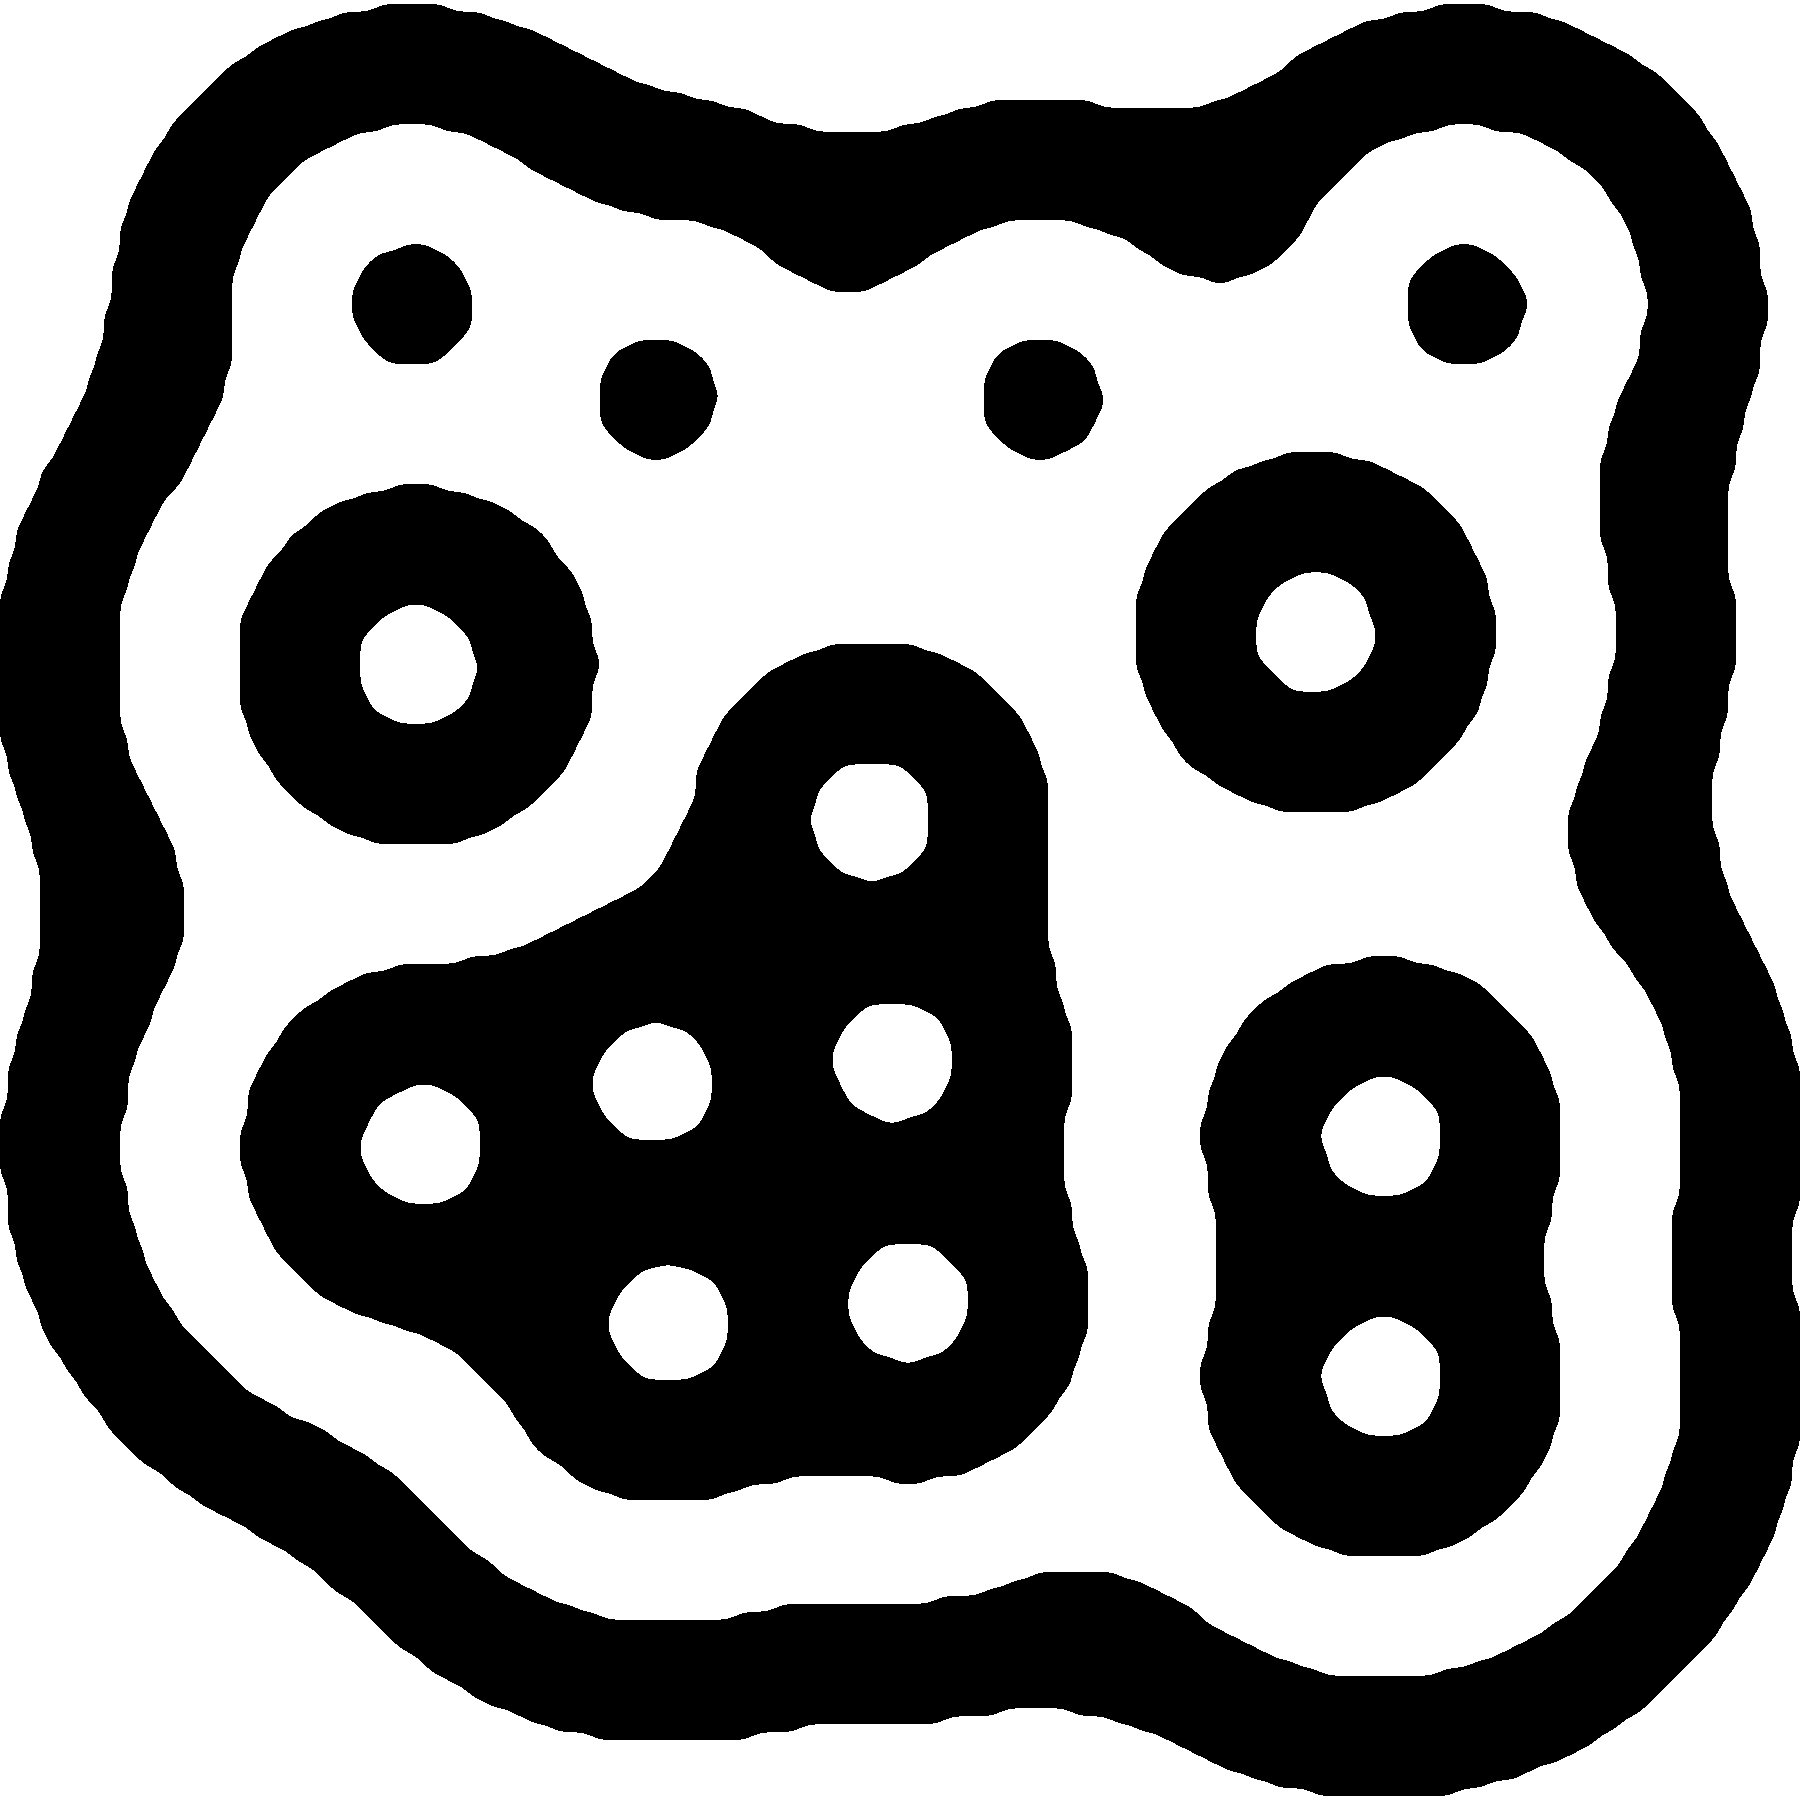
\includegraphics[height=1in]{img/ImplementierungInput/ReactivisionCode.png}
	\caption{ReacTIVision Code}
	\label{fig:img_ImplementierungInput_ReactivisionCode}
\end{figure}

Die ReacTIVision-Software ist plattformübergreifend für Windows, Linux und Mac OS X verfügbar. Sie greift über plattformspezifische Schnittstellen auf angeschlossene Kamera zu und wertet das empfangene Bild in Echtzeit aus. Dabei sind bei einer Kameraauflösung von 1024 x 68 Bildpunkten Bildraten von 15-20 Bildern pro Sekunde erreichbar. Diese Leistung wird auch durch eine höhere Anzahl von gleichzeitig im Bild vorhandenen Codes nicht merklich geringer.

Neben der Position der Codes wird auch deren aktuelle Rotation sowie die erste Ableitung dieser drei Parameter (also ein Maß für die Bewegung) extrahiert. Zudem können Finger, die die Oberfläche berühren erkannt und deren Position extrahiert werden. Dies ist auch für mehrere Finger möglich, wobei eine eindeutige Zuordnung über die Zeit erhalten bleibt und so rudimentäre Multitouch-Funktionen umgesetzt werden können.

Als problematisch stellt sich wie auch bei allen anderen betrachteten optischen Ansätzen die Abhängigkeit der Erkennungsqualität von der Umgebungsbeleuchtung bzw. deren Änderung dar. ReacTIVision arbeitet mit adaptiven Filteralgorithmen zur Aufbereitung des Bildes, was jedoch nur leichte Beleuchtungsschwankungen ausgleichen kann. Die Software kann händisch an die Beleuchtungsverhältnisse angepasst werden (Einstellung der Blendenöffnung und der Bildverstärkung), bei sich ändernden Lichtverhältnissen muss jedoch regelmäßig eine manuelle Nachführung der Parameter vorgenommen werden.

Die aus dem Bilderstrom gewonnenen Daten werden im Falle einer Änderung zumindest eines Wertes über ein Netzwerkschnittstelle (UDP-basiert) in einem propritären Protokoll zur Verfügung gestellt. Zu diesem Protokoll werden Schnittstellen und Referenzimplementierungen in unterschiedlichen Programmiersprachen, unter anderem C(++) und Java, zur Verfügung gestellt. Applikationen können diese Schnittstelle implementieren und werden sie mittels insgesamt sechs zu implementierenden Methoden an die Erkennungsroutinen angebunden (3 für Code- und 3 für Fingertracking).

% paragraph reactivision (end)

% subsubsection frameworks_für_video_basierten_input (end)

% subsection verfügbare_frameworks (end)

\subsection{Technologieentscheidung} % (fold)
\label{sub:technologieentscheidung}

Auf Basis der Anforderungen, die im Anwendungsfall an das Werkzeug gestellt werden, ist nun nach der grundsätzlichen Entscheidung für ein auf optischen Ansätzen basierenden System die Entscheidung für ein konkretes Framework zu treffen. 

\subsubsection{Vergleich der Frameworks für videobasieren Input}\label{subs:vergleich_video_frameworks}

Für die Anbindung von videobasiertem Input wurde drei Frameworks vorgestellt. Diese Frameworks sind nun hinsichtlich mehrere Aspekte zu vergleichen, die sich aus den Anforderungen der zu erstellenden Applikation sowie der Forderung nach möglichst einfacher (im Sinne von unaufwändiger) Einbindung des Frameworks ergeben. Im Einzelnen sind dies 
\begin{itemize}
	\item die Unterstützung bei der Einbindung von Kameras, eine Schnittstelle zur Programmiersprache Java,
	\item eine stabile und in Echtzeit ablaufende Bilderkennung,
	\item eine ausreichende Anzahl von Codes (Größenordnung 100),
	\item die Extraktion von Position und Rotationsinformation für Codes im Erfassungsbereich der Kamera sowie
	\item die technische und lizenzrechtliche Möglichkeit, die Frameworks an die eigenen Anforderungen anzupassen.
\end{itemize}
    
ReacTIVision bietet die umfassendste Unterstützung zur Einbindung unterschiedlicher Videoquellen und ist zur Anwendungsseite hin durch die Netzwerkschnittstelle am flexibelsten einsetzbar. Alle drei Ansätze bieten Schnittstellen bzw. Konnektoren für die Programmiersprache Java an. Die Frameworks selbst sind in C(++) oder Java erstellt und können auf den gängigen Plattformen (Windows, Linux, Mac OS x) ausgeführt werden. Eine Verteilung der Applikation auf mehrere Rechner wird nur von ReacTIVision explizit unterstützt.

Hinsichtlich der eigentlichen Bilderkennungs-Routinen sind die Ansätze in ihrer Leistung und Geschwindigkeit vergleichbar, leiden aber alle unter der Abhängigkeit von der Umgebungsbeleuchtung. ReacTIVision bietet hier als einziger Ansatz die Möglichkeit, Kameraparameter zur Laufzeit nachzuführen und so Schwankungen der Umgebungshelligkeit auszugleichen.

Durch den eingesetzten Mapping-Ansatz sind ARToolkit und ReacTIVision hinsichtlich Form und Inhalt der Codes flexibler als direkt codierende Ansätze wie Visual Codes. Dies ist im konkreten Anwendungsfall relevant, da aufgrund der Token-Form und deren beschränkter Größe eine ideale Platzausnutzung erfolgen muss, um ausreichende Erkennungsleistung zu gewährleisten.

Die Extraktion der Raumparameter (Neigungsinformation, ...), die von ARToolkit und Visual Codes ermöglicht wird, ist in bei tisch-basierten Werkzeugen wie dem hier vorgestellten nicht notwendig - die Erhebung planarer Parameter (Position und Rotation) ist ausreichend.

Die Anzahl der verfügbaren und zuverlässig unterscheidbaren Codes muss für die hier vorgeschlagene Anwendung in der Größenordnung 100 liegen. Visual Codes und ReacTIVision erfüllen diese Anforderung, ARToolkit bietet im Lieferumfang weniger Codes an, diese können jedoch erweitert werden und bieten auch in der gerforderten Anzahl noch ausreichend Unterscheidungsmerkmale für eine zuverlässige Unterscheidung (REF Schmalstieg TU System).

Von allen drei Systemen steht der Source-Code zur Verfüng. Lizenzrechtlich erlauben ebenfalls alle Systeme eine Veränderung des Sourcecode (LIZENZEN AUFZÄHLEN)

\begin{center}
	\begin{tabular}{| p{3cm} || p{3cm} | p{3cm} | p{3cm} |} \hline
		 & ARToolkit & Visual Codes & ReacTIVision \\ \hline \hline
		Kamera\-unterstützung 		  		& ? & nativ nur für Mobiltelefone & nativ auf allen unterstützten Plattformen via USB und Firewire \\ \hline
		Plattformen 			  	  		& x & Java-basiert auf allen Plattformen & Windows, Linux, Mac OS X \\ \hline
		Schnittstelle zu Java 		  		& ja & ja & ja \\ \hline
		Stabilität der Bilderkennung 	  	& eher hoch & eher hoch & hoch \\ \hline
		Geschwindigkeit der Bilderkennung 	& > 10 fps & > 10 fps & > 10 fps \\ \hline
		Anzahl von Codes 		  			& eher hoch & hoch & hoch \\ \hline
		Erkennung von Position 		  		& ja & ja & ja \\ \hline
		Erkennung von Rotation 				& ja & ja & ja \\ \hline
		Source-Code verfügbar 			  	& ja & ja & ja \\ \hline
		Lizenz 				 				& ? & ? & ? \\ \hline
	\end{tabular}
\end{center}

Auf Basis dieses Vergleichs ist erkennbar, dass das ReacTIVision-Framework für den hier verfolgten Ansatz am besten geeignet erscheint. Es wird deshalb zur Umsetzung des Werkzeugs verwendet. Der zusätzliche Einsatz eines generischen Frameworks zur Flexibilisierung der Applikationsstruktur ist damit nach wie vor möglich und wird im nächsten Abschnitt diskutiert.

% subsubsection vergleich_video_frameworks (end)

\subsubsection{Vergleich der generischen Frameworks}\label{subs:vergleich_generische_frameworks}

Der Einsatz eines generischen Frameworks ist im konkreten Anwendungsfall für die Modularisierung der Interpretations- und Output-Module denkbar. Eine weitere Anwendung von generischen Frameworks ist die Anforderung nach der Skalierbarkeit der Anzahl der Ausgabemodule ggf. auch während des Betriebs der Applikation (um z.B. weitere Viewer-Module zur Beobachung des Modellierungsvorganges während der Laufzeit zuschalten zu können). Die Aspekte die beim Vergleich der vorgestellten Ansätze berücksichtigt werden müssen, sind deshalb
\begin{itemize}
  	\item die Unterstützung von modularen funktionalen Einheiten sowie
	\item die Möglichkeit diese zur Laufzeit zu laden und entfernen und
	\item die Konfigurierbarkeit der Verknüpfungen dieser Module.
	\item Daneben sind nicht-funktionale Anforderungen wie Skalierbarkeit und
	\item Effizienz bei der Weiterleitung und Verteilung der Anwendungsdaten 
\end{itemize}  
zu berücksichtigen.

Die Modularisierung der Applikation wird von allen vier vorgestellten Frameworks unterstützt. Das Context Toolkit, Papiermaché und TUIpist unterscheiden dabei konzeptuell zwischen unterschiedlichen Arten von von Modulen (im Wesentlichen "Input", "Verarbeitung" und "Output"), das SiLiCon Context Framework unterscheidet nicht zwischen unterschiedlichen Modultypen, dort wird die Rolle eines Moduls ausschließlich über seine Attribute (also die nach außen sichtbaren funktionalen Einheiten) definiert.

Eine Erweiterbarkeit der Applikation zur Laufzeit ist nur beim SiLiCon Context Framework und bei TUIpist möglich. DAs SiLiCon Context Framework arbeitet hier mit eigens erstellten Java-Classloadern, die das Nachladen von Klassen (Modulen) und deren Integration in die Infrasturktur erlauben. TUIpist verwendet die inhärent dynamische Erweiterbarkeit des Java Jini (REF) Frameworks, auf Basis dessen es implementiert wurde. Das Context Toolkit und Papiermaché erlauben kein Nachladen oder Entfernen funktionaler Einheiten während der Laufzeit.

Die Konfiguration der Verbindungen zwischen den Modulen ist bei allen Frameworks möglich, konzeptuell jedoch unterschiedlich ausgeführt. Im Context Toolkit und in Papiermaché muss die Verbindung direkt im Programmcode codiert werden und wird im wesentlichen auf Methodenaufrufe abgebildet. Das SiLiCon Context Framework verwendet ereignisbasierte Regeln, um Module zu verknüpfen. Ein von einem Modul ausgelöstes Ereignis kann hier (ggf. durch Bedingungen eingeschränkt) Aktionen in anderen Modulen auslösen. Eine Besonderheit dieses Ansatzes ist, das Teile der Interpretationslogik (also der Erkennung von Benutzerinteraktion aus den Rohdaten) in die Regeln ausgelagert werden und damit jederzeit dynamisch verändert werden können. So kann zum Beispiel die Interpretation der Nähe zwischen zwei Token in einer Regel codiert werden und so in die Reihe der zulässigen (bzw. erkennbaren) Interaktionen aufgenommen werden. TUIpist benötigt hingegen keinerlei explizite Verbindung der Module, da sämtliche Koordination über den geteilten Datenraum ausgeführt wird. Die Verknüpfungslogik wird hier in die Module verschoben, die selbst wissen müssen, für welche Daten für sie ggf. relevant sind und welche sie deshalb dem Tuplespace entnehmen.

Hinsichtlich der Skalierbarkeit der Frameworks können aufgrund mangelnder Vergleichsdaten keine fundierten Aussagen getroffen werden. Hinzuweisen ist jedoch auf die Unterstützung von verteiltem Betrieb einer Applikation durch das SiLiCon Context Framework (via SOAP-Aufrufe (REF) und das TUIpist Framework (via Jini und Java RMI (REF)). Durch diese Verteilbarkeit ist kann die Problematik mangelnder Rechenressource umgangen werden, die vorallem bei rechenintensiven Anwendungen wie der eingesetzten Bildanalyse im optischen Tracking auftritt.

Die Beurteilung der Effizienz der Frameworks ist hier in Hinblick auf die geforderte Echtzeit-Interaktion mit dem System als relevant zu erachten. Das Haupt-Kriterium für Effizienz ist dementsprechend die Verzögerung zwischen Eingabe-Ereignissen und dem Feedback auf Applikationsebene, die beim Einsatz der Frameworks auftritt. Eine Beurteilung in absoluten Zahlen kann hier mangels entsprechenden Datenquellen ebenfalls nicht erfolgen, konzeptuell sind aber bei den Frameworks, in denen Module direkt durch Programm-Code verknüpft werden (Context Toolkit und Papiermaché), eher geringe Verzögerungen zu erwarte. Die beiden Frameworks, die mit expliziter und konfigurierbarer Middleware zur Datenvermittlung arbeiten (SiLiCon Context Framework und TUIpist) lassen eher höhere Verzögerungen erwarten, wobei der ereignisbasierte Ansatz des SiLiCon Context Framework dem daten-basieren Ansatz von TUIpist insofern überlegen ist, als das bei der datenbasierten Interaktion die Module in regelmäßigen Intervallen nach neuen Daten suchen müssen (Polling, Information Pull-Ansatz), während bei ereignisbasierten Ansätzen die Benachrichtung der betroffenen Module automatisch und zum Zeitpunkt des Auftretens des Ereignisses erfolgt (Information Push-Ansatz). Der Information Pull-Ansatz sorgt dabei einerseits für erhöhten Kommunikationsaufwand und potentiell für Verzögerungen bei Ereignissen, die innerhalb eines Polling-Intervalls auftreten.

-- VERGLEICHSTABELLE --

Auf Basis dieser Gegenüberstellung erscheinen das SiLiCon Context Framework und TUIpist als die beiden geeignetsten Kandidaten für den Einsatz als generisches Framework im hier vorgestellten Anwendungsfall. Das Context Toolkit und Papiermaché scheiden aus verschiedenen Gründen, vorallem aber der mangelnden Flexiblität aus.

Stellt man die beiden verbleibenden Frameworks gegenüber, so sind hinsichtlich der funktionalen Anforderungen keine Vorteile für einen der beiden Kandidaten zu identifizieren. Hinsichtlich der nichtfunktionalen Anforderungen scheint TUIpist hinsichtlich der Skalierbarkeit leichte Vorteile zu haben, da das Nachladen von neuen Instanzen weniger Aufwand versacht als im Fall des SiLiCon Context Framework (lediglich Laden eines Moduls im ersten Fall gegenüber Laden und Einbinden über eine Änderung der Regelbasis im zweiten Fall). Außerdem ist die technologische Basis der Verteilungsarchitektur in TUIpist konzeptionell auf höherer Ebene angesiedelt und mächtiger in der Verwaltung der Applikationsstruktur (unter anderem werden neue Module bei TUIpist automatisch in die Infrastruktur eingebunden, sobald sie angemeldet werden, im SiLiCon Context Framework muss für jeden Kommunikationskanal die IP-Adresse des Empfängers bekannt sein und in die Regelbasis aufgenommen werden). 

Hinsichtlich der Effizienz der Kommunikation bietet das SiLiCon Context Framework gegenüber TUIpist aus den oben beschriebenen Gründen (Benachrichtung über Änderungen gegenüber Polling) Vorteile. Für die hier beschriebene Applikation fällt die Entscheidung trotzdem zugunsten TUIpist. Neben der generell unaufwändigeren Konfigurierbarkeit kommt die Struktur von TUIpist einem iterativen Software-Entwicklungsprozess insofern eher entgegen, als dass die Modularisierung von initialen, monolithischen Prototypen (z.B. basierend auf der Struktur des zuvor ausgewählten ReacTIVision-Frameworks) einfacher möglich ist. Dies liegt darin begründet, dass in der modularen und dynamischen Struktur von TUIpist die gesamte Applikationslogik in den Modulen enthalten ist und so Teile aus einer monolithischen Applikation herausgelöst und direkt übernommen werden können, wobei lediglich die Logik der Datenübergabe von direkten Methoden-Aufrufen auf die TUIpist-Routinen zum Zugriff auf den Tuplespace umgearbeitet bzw. erweitert werden muss. Beim korrekten Einsatz des SiLiCon Context Framework wandert wie oben beschrieben ein Teil der Applikationslogik in die Regelbasis, was erhöhten Aufwand bei der iterativen Entwicklung verursacht und außerdem das Zusammenspiel der Applikations-Module unübersichtlicher und schwerer fassbar macht.

% subsubsection vergleich_generische_frameworks (end)

% subsection technologieentscheidung (end)
% section möglichkeiten_zur_erfassung_von_benutzerinteraktion (end)

\section{Konzeption und Umsetzung der Hardwarekomponenten} % (fold)
\label{sec:konzeption_und_umsetzung_der_hardwarekomponenten}

Basierend auf der oben getroffenen Techhnologieentscheidung zugunsten eines optischen, video-basierten Input-Systems für das hier zu erstellende Tabletop Interface wird in diesem Abschnitt das konkrete Hardware-Design beschrieben. Dies umfasst die Beschreibung des Tabletop Interfaces im Überblick und detaillierte Betrachtungen des Token-Designs sowie der Tisch-Oberfläche, die als Input-Kanal dient. Im weiteren werden spezifische Herausforderungen und der jeweilige hier verfolgte Lösungsansatz beschrieben. Nicht Gegenstand dieses Abschnitts sind jene Hardware-Komponenten, die für die Ausgabe von Information eingesetzt werden. Obwohl hier im Überblick angeführt, werden sie detailliert erst in Kapitel XY über die Visualisierung der Modellierungsinformation beschrieben.

\subsection{Überblick} % (fold)
\label{sub:Überblick}

Das Tabletop Interface ist als Tisch mit einer Oberfläche von 100 cm x 80 cm ausgeführt. Die Höhe beträgt 110 cm. Die wesentlichen Hardwarekomponenten sind die Tischoberfläche, die in semi-transparenten Acrylglas ausgeführt ist und die Bodenplatte, in die die Kamera zum optischen Tracking der Tokens auf der Oberfläche sowie der Videoprojektor zur Ausgabe von Information auf der Oberfläche (Projektion von unten) eingebaut sind (siehe Abbildung \ref{fig:img_ImplementierungInput_TischSeitenansicht}). Der Tisch ist auf allen Seitenflächen mit Platten aus Styropor (MARKENNAME -> KUNSTSTOFF) verkleidet, um im Inneren kontrollierte Umgebungslichtbedingungen für die Bilderfassung mit der Kamera zu schaffen. Die kontrollierten Bedingungen werden durch den Einsatz von vier Beleutungsmodulen gewährleistet, die ebenfalls in der Bodenplatte integriert sind und über den Seitenflächen eingebaute Streuscheiben für eine einheitliche, diffuse Beleuchtung der Tischinnenraums sowie der Oberfläche sorgen.

\begin{figure}[htbp]
	\centering
		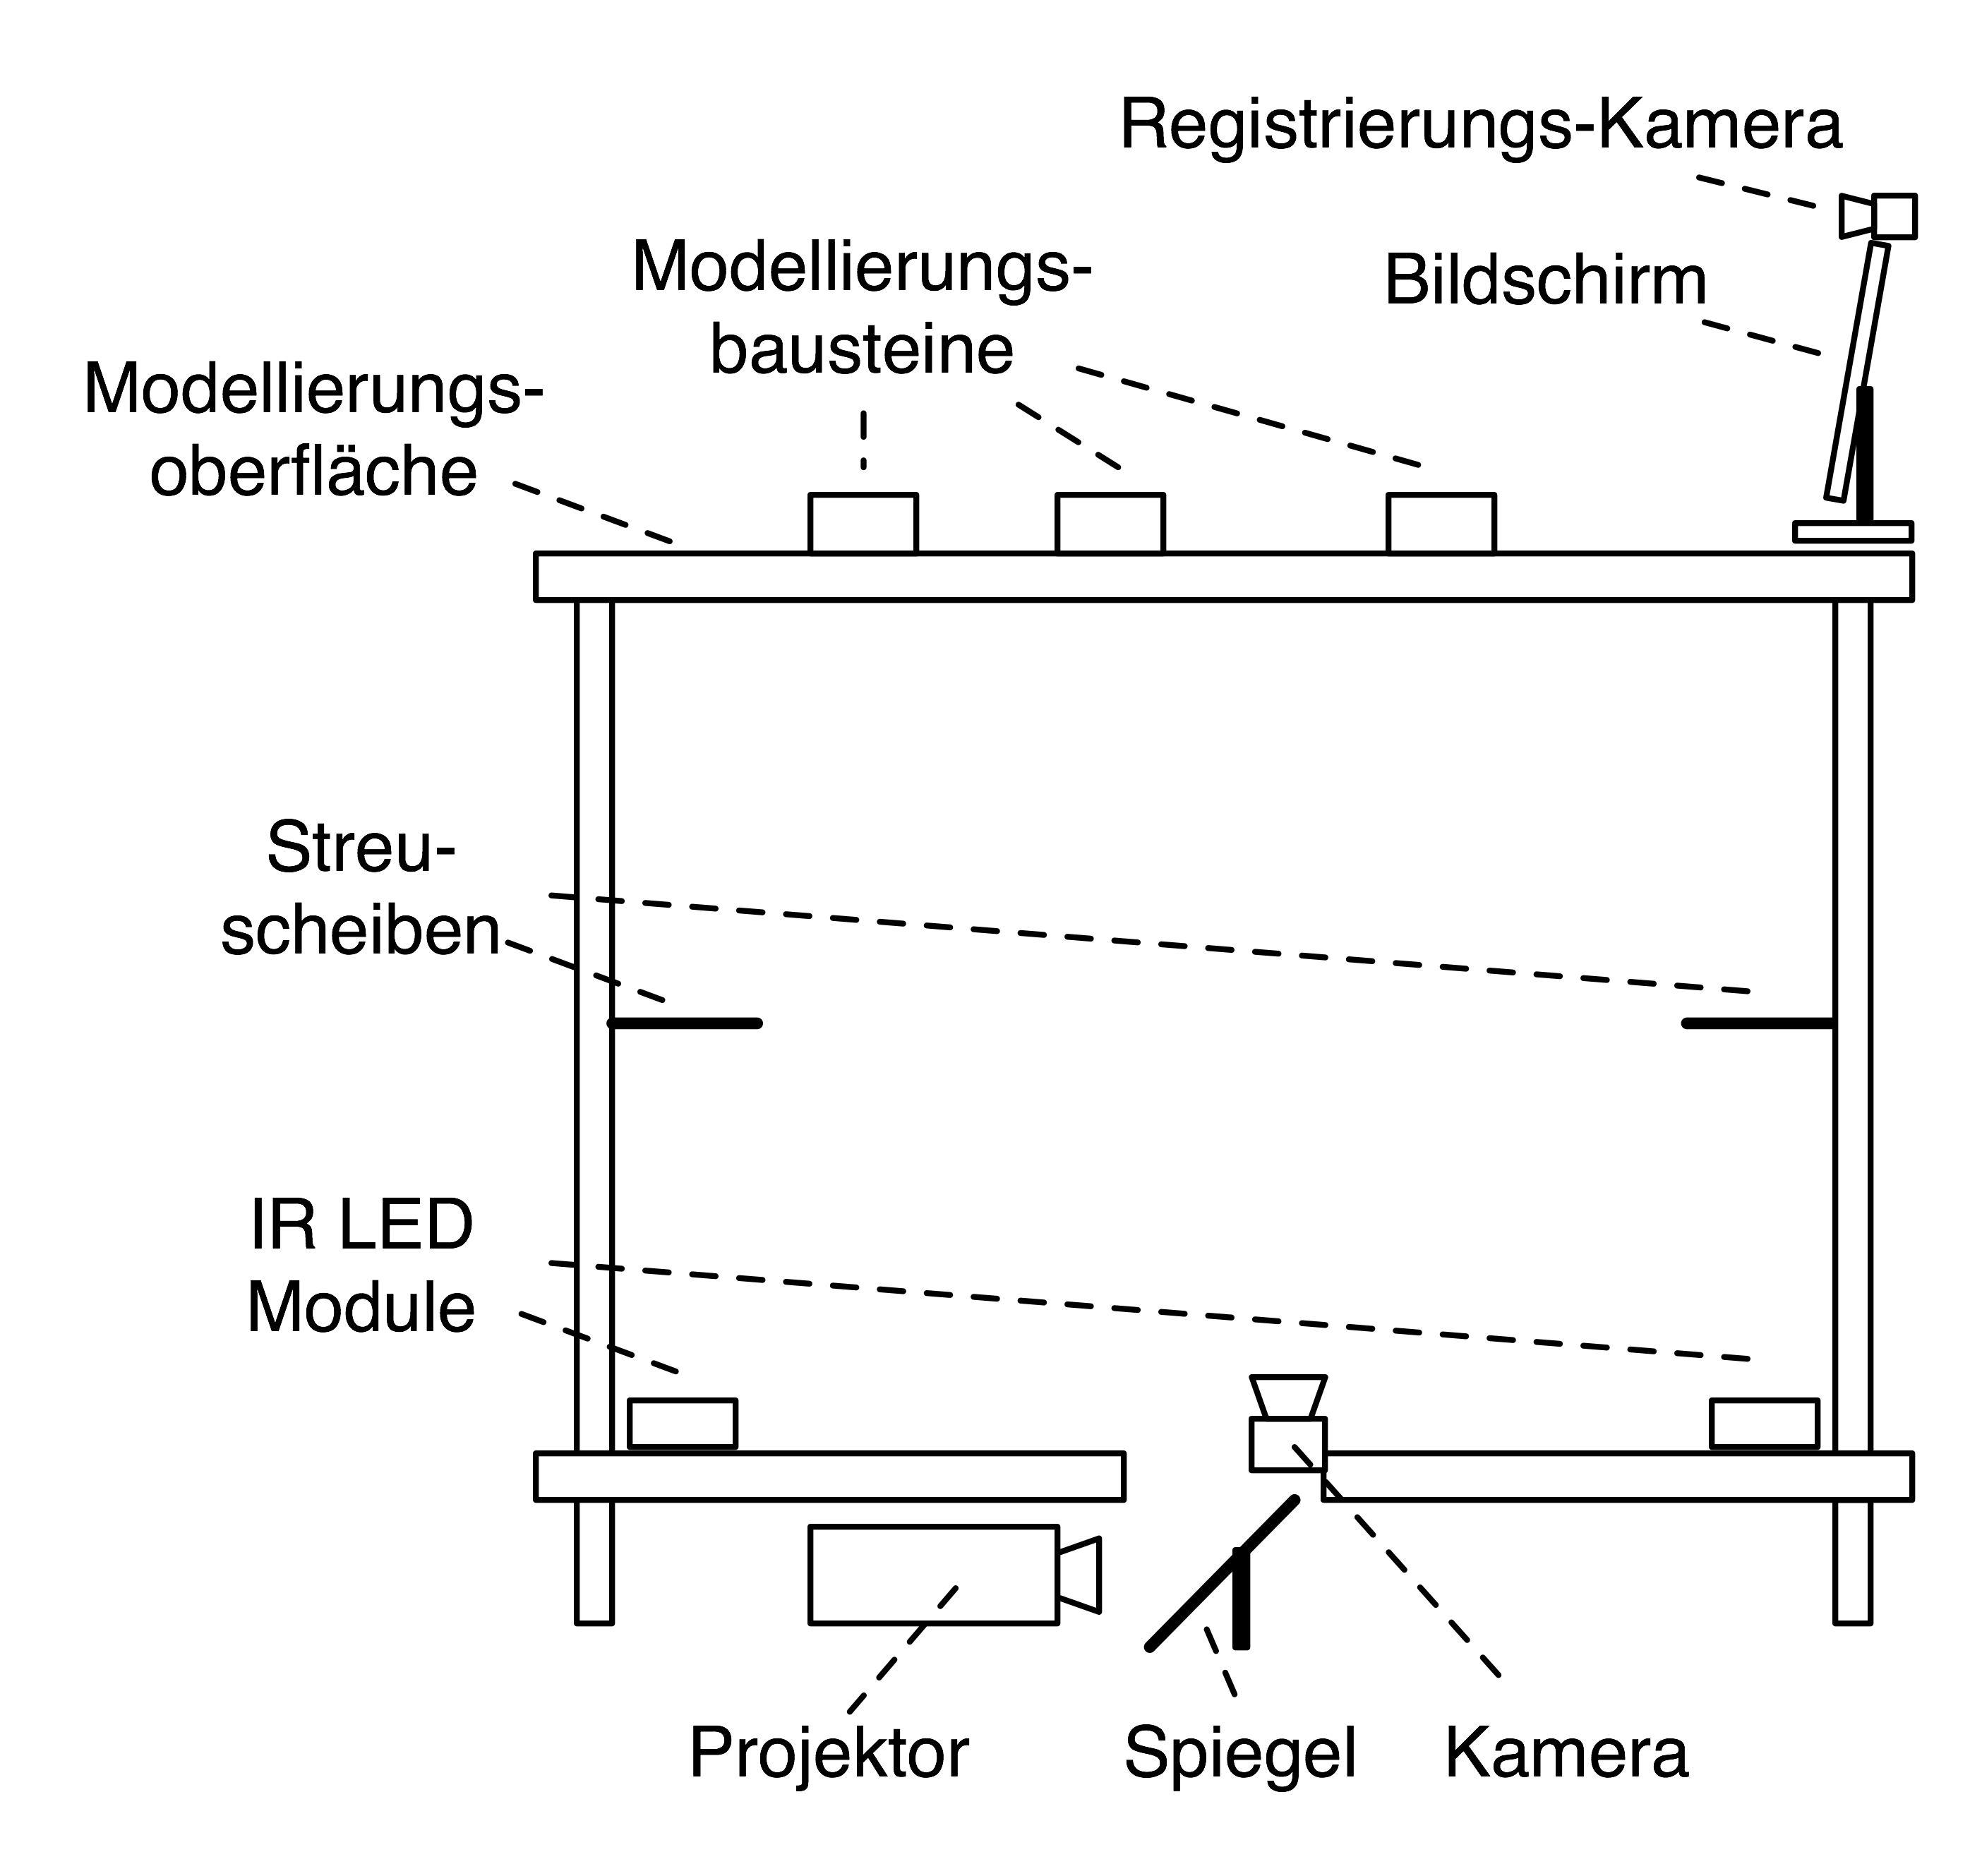
\includegraphics[height=4in]{img/ImplementierungInput/TischSeitenansicht.png}
	\caption{Überblick über den Aufbau des Tabletop Interfaces}
	\label{fig:img_ImplementierungInput_TischSeitenansicht}
\end{figure}

Am Tisch befindet sich zusätzlich ein Bildschirm, auf dem entsprechend der Anforderungen zur Unterstützung der Modellierung Zusatzinformation ausgegeben wird. Eine zweite Kamera, die am Bildschirm sitzt und der unterstützenden Erfassung von Information dient (zum Beispiel der Registrierung von geschachtelten Token wie oben bereits beschrieben).

Das gesamte System ist so zerlegbar, dass es im Kofferraum eines Mittelklassewagens transportiert werden kann. Es werden dazu die Verkleidungsplatten und Tischbeine entfernt, die Tischplatte kann dann direkt auf die Bodenplatte gesetzt und verbunden werden. Das Volumen reduziert sich dabei auf 100 cm x 80 cm x 20 cm, wobei die Tischbeine, die Verkleidungsplatten und der Videoprojektor separat transportiert werden müssen. Ein Zusammenbau des Systems inklusive Kalibrierung der Eingabe- und Ausgabe-Kanäle ist in etwa 30 Minuten möglich.

% subsection Überblick (end)

\subsection{Tokens \& Input-Werkzeuge} % (fold)
\label{sub:tokens_&_input_werkzeuge}

In diesem Abschnitt werden die einzelnen durch die Benutzer manipulierbaren Token-Árten beschrieben. Neben den eigentlichen Modellierungstokens sind dies die Tokens zur Einbettung in Container sowie die Werkzeugtokens, von denen es Ausführungen zur generischen Interaktion mit dem System und Tokens zur Auslösung bzw. Kontrolle spezifischer Funktionalitäten gibt.

\subsubsection{Modellierungs-Tokens} %fold 
\label{subs:modellierungs_tokens}

Die eingesetzten Modellierungs-Tokens sind aus nicht transparentem Acrylglas gefertigt. Ihre Außenmaße betragen in etwa (je nach Form) 10 cm x 6 cm in der Grundfläche und 4 cm in der Höhe. Damit ist einerseits eine ausreichende Größe zur Anbringung der ReacTIVision-Codes gewährleistet, andererseits sind noch klein genug, um in einer Hand gehalten und manipuliert werden zu können. Die Codes werden auf der Unterseite der Tokens angebracht und auch von unten erfasst (siehe nächster Abschnitt), um eine Verdeckung der Codes während der Manipulation zu verhindern (siehe Abbildung \ref{fig:img_ImplementierungInput_TokensCodes}).

\begin{figure}[htbp]
	\centering
		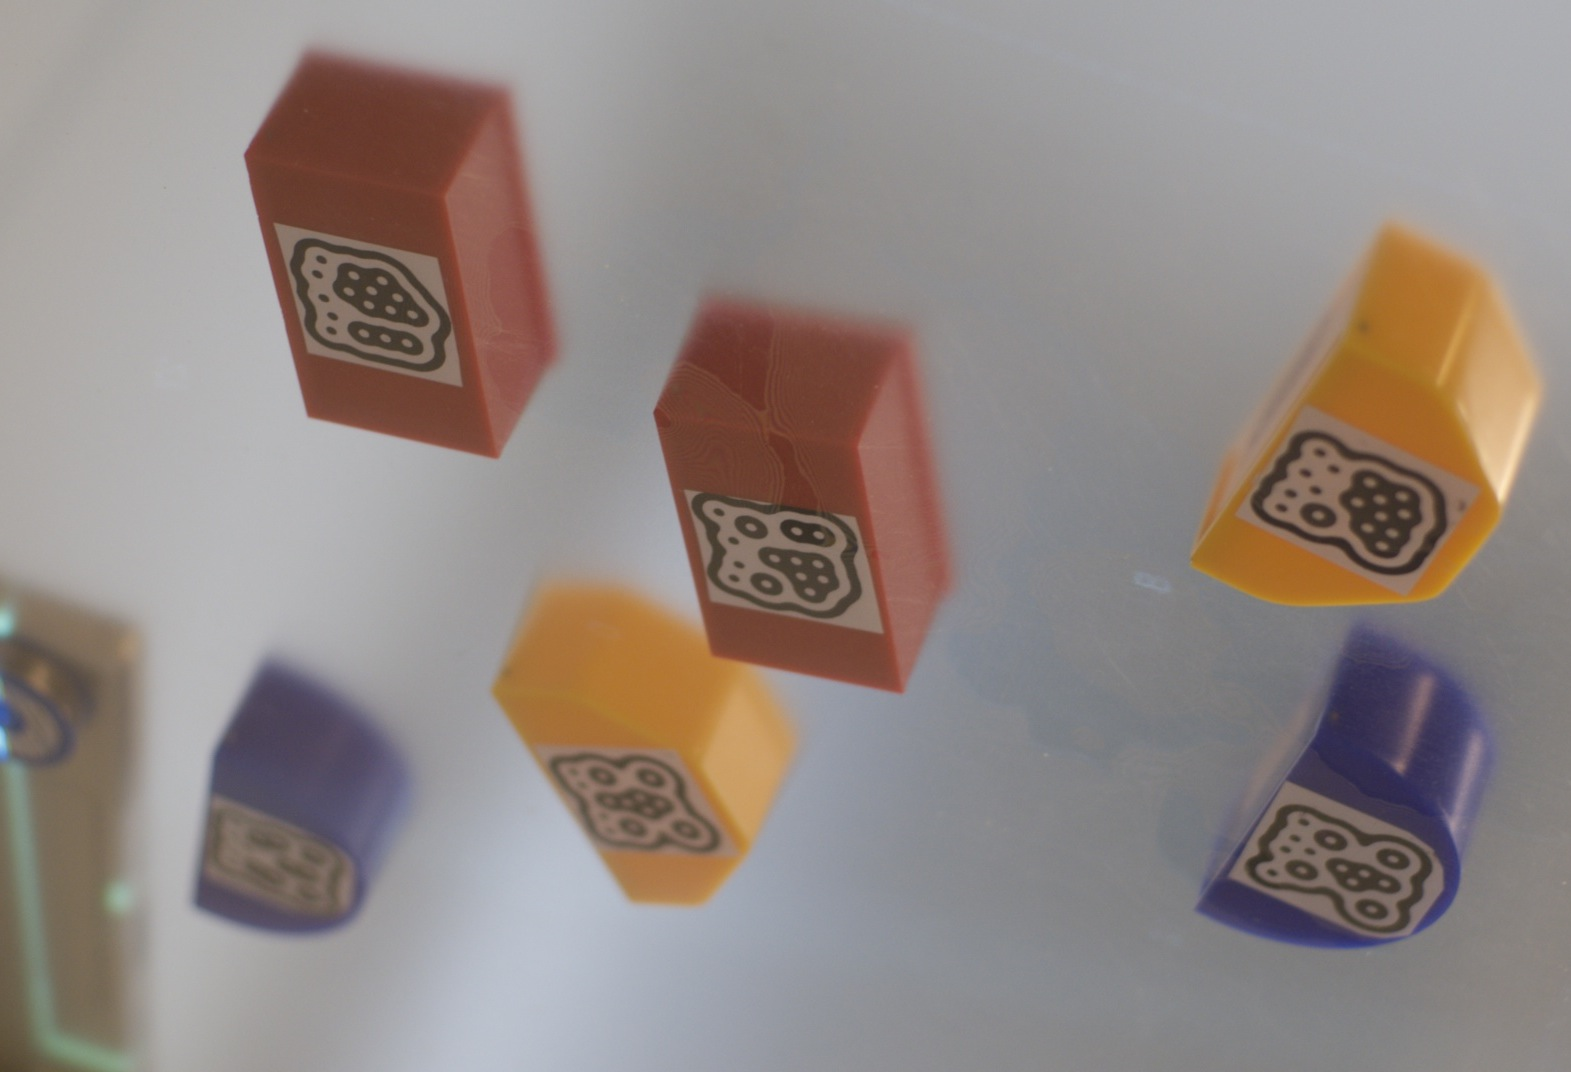
\includegraphics[height=2in]{img/ImplementierungInput/TokensCodes.jpg}
	\caption{An Tokens angebrachte ReacTIVision-Codes zur Identifikation}
	\label{fig:img_ImplementierungInput_TokensCodes}
\end{figure}

\begin{figure}[htbp]
	\centering
		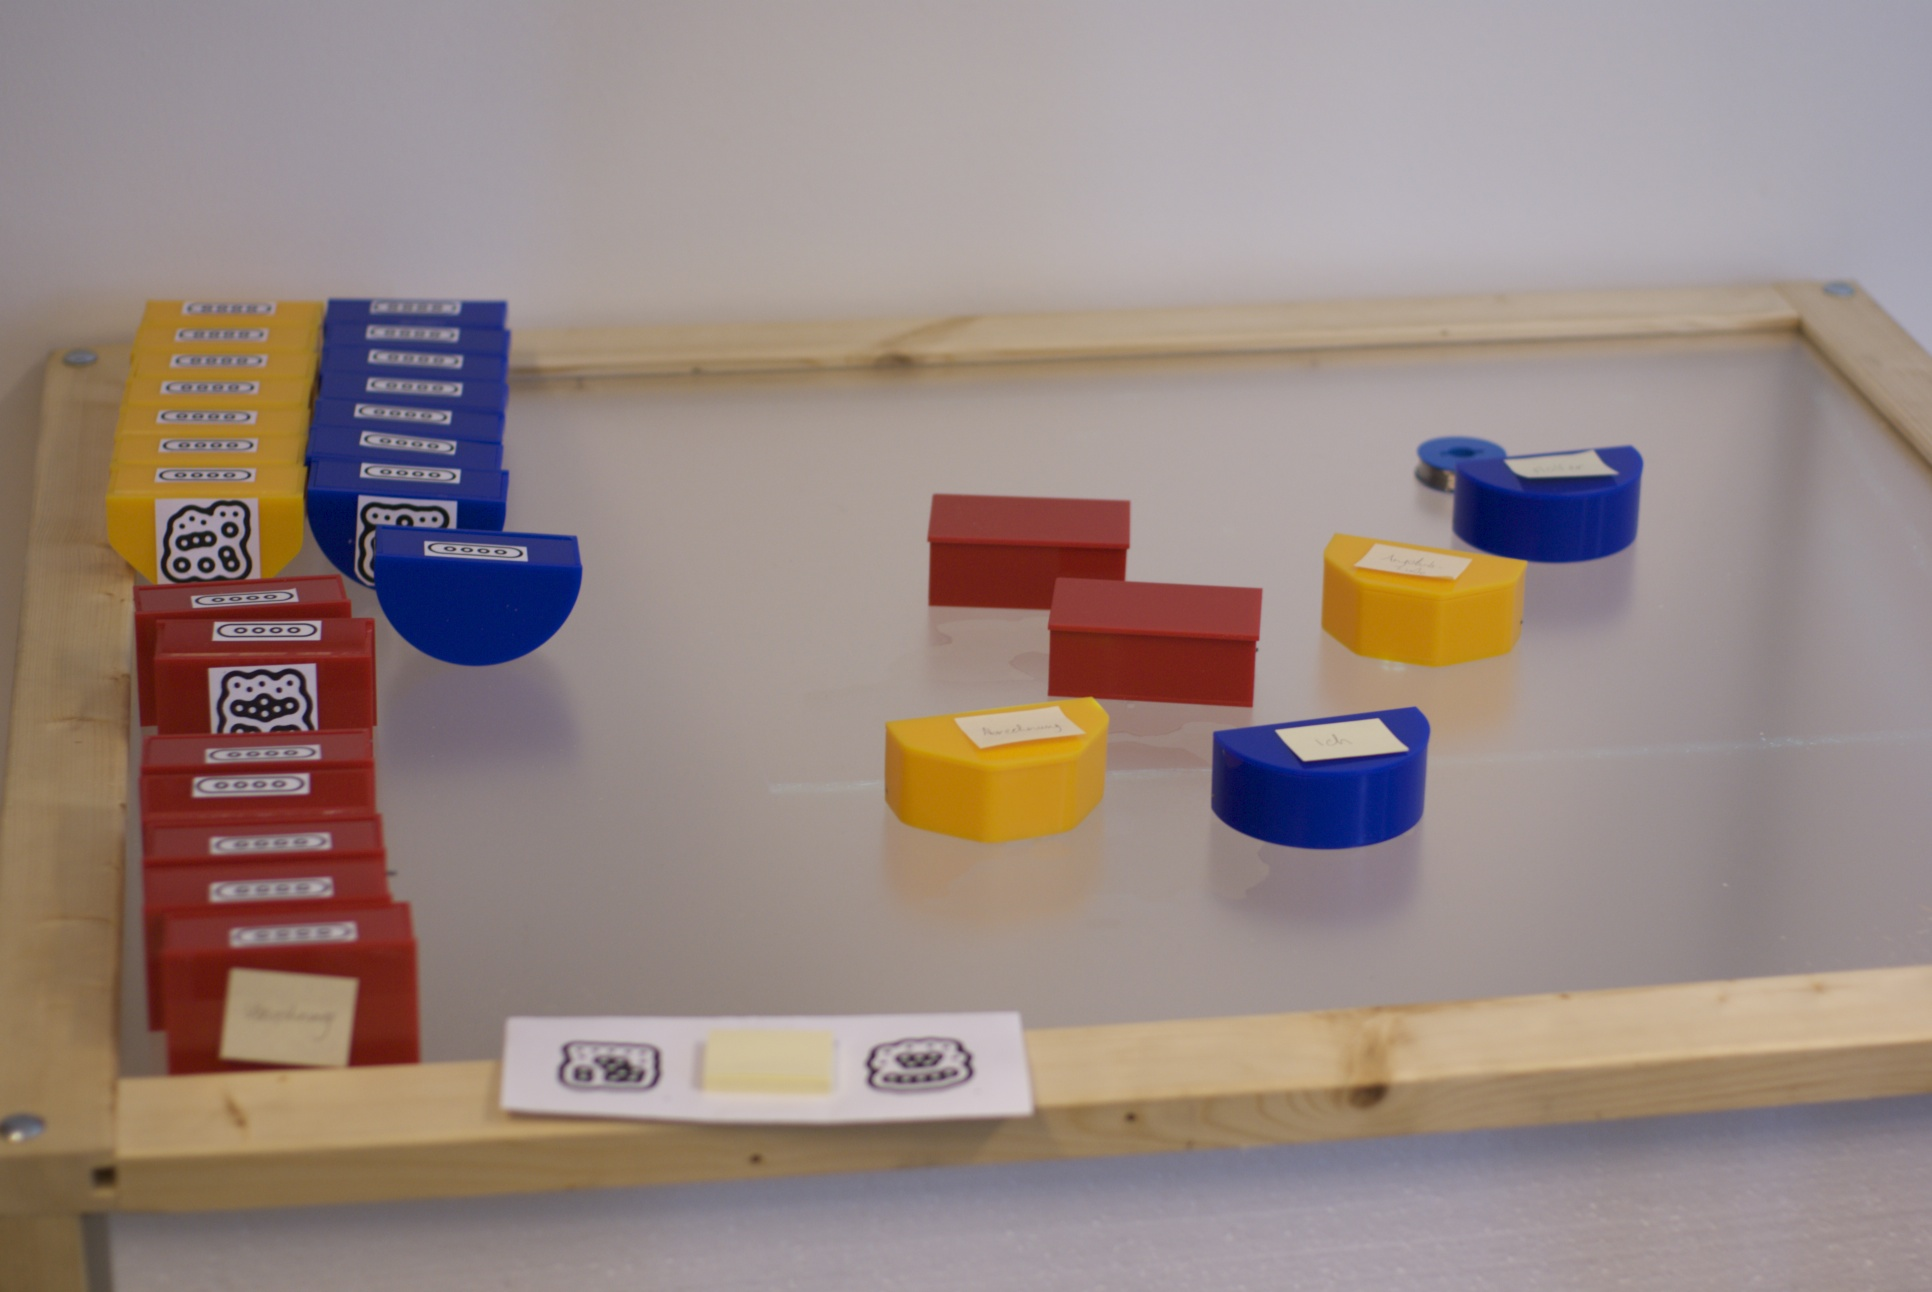
\includegraphics[height=2in]{img/ImplementierungInput/TokenTypes.jpg}
	\caption{Arten von Modellierungstokens}
	\label{fig:img_ImplementierungInput_TokenTypes}
\end{figure}


Die Modellierungs-Tokens wurden in drei Ausführungen gefertigt (siehe Abbildung \ref{fig:img_ImplementierungInput_TokenTypes}). Diese unterscheiden sich in Form und Farbe und können während der Modellierung von den Benutzern frei mit Bedeutung belegt werden. Die Auswahl der Formen und Farben erfolgte inspiriert von den Symbolen gängiger Modellierungsnotationen in Abstimmung mit fertigungstechnischen Einschränkungen. Eine wie in XY (REF von TEI) vorgeschlagene Analyse geeigneter Token-Formen und eine auf diesen Ergebnissen basierende Umsetzung wurde nicht vorgenommen. Die liegt vor allem in der Tatsache begründet, dass sich der Fokus der hier vorgestellten Arbeit im Entwicklungsprozess von einem Werkzeug zur Geschäftsprozessmodellierung (mit vorgegebener Notation) hin zu einem allgemeiner einsetzbaren Werkzeug zur generischen Modellierung konzeptueller Modelle (ohne vorgegebene Notation) entwickelte. Die Auswahl der Token-Formen fiel in die erste Phase, wodurch die Tokens im äußeren Erscheinungsbild an gängige Notationen zur Ablauf-Modellierung angelehnt sind. Die Auswirkung der Token-Form auf die Modellierung scheint aber bei Benutzern ohne Modellierungs-Vorbildung geringen bis keinen Einfluss auf den Modellierungsprozess zu haben (siehe Kapitel XY - Evaluierung).

\begin{figure}[htbp]
	\centering
		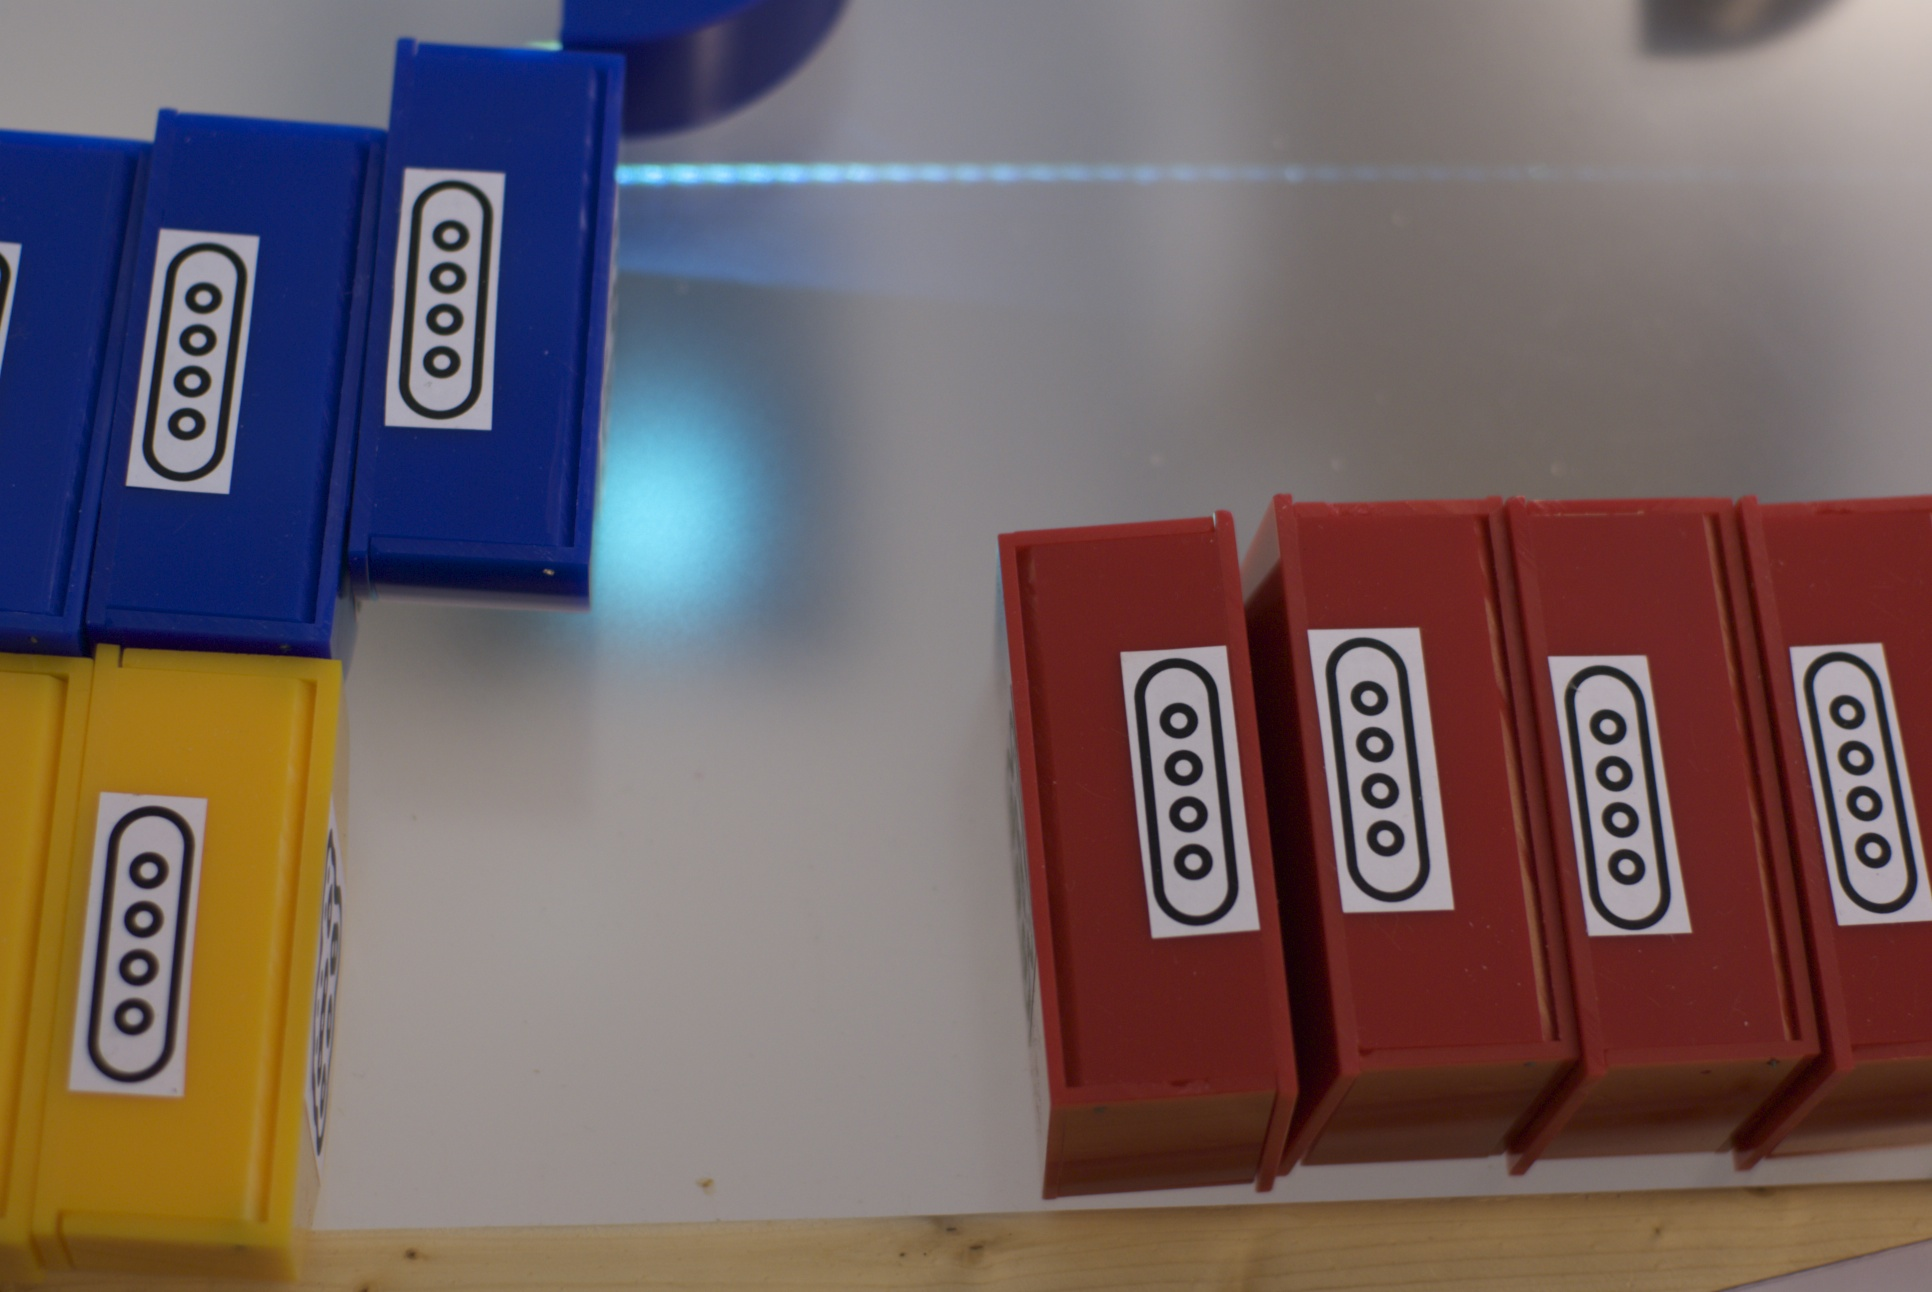
\includegraphics[height=2in]{img/ImplementierungInput/ContainerRueckseite.jpg}
	\caption{Rückwand von Container Tokens}
	\label{fig:img_ImplementierungInput_ContainerRueckseite}
\end{figure}

Wie in der Beschreibung der Anforderungen gefordert und oben bereits beschrieben sind die Modellierungs-Tokens als Container ausgeführt. Im Abschnitt über die Erkennung des Token-Zustands (REF) wurde beschrieben, das beim Einsatz von optischem Tracking eine Möglichkeit geschaffen werden muss, im Kamerabild zu erkennen, ob ein Token geöffnet ist oder nicht. Um den konsequenten Einsatz eines Erkennungsframeworks (ReacTIVision) zu gewährleisten, wird zu diesem Zweck ein zweiter Code eingesetzt (siehe Abbildung \ref{fig:img_ImplementierungInput_ContainerRueckseite}), der nur dann für die Kamera sichtbar wird, wenn das Token geöffnet ist. Hardwareseitig ist dies so umgesetzt, das die Modellierungstokens einen Öffnungsmechanismus besitzen, dessen Schanier nicht am Deckel sitzt (und damit nur diesen beweglich machen würde), sondern an der Bodenplatte, wodurch sich beim Öffnen eines Containers nicht nur der Deckel sondern auch die Hinterwand des Tokens bewegt (siehe Abbildung \ref{fig:img_ImplementierungInput_ContainerToken}). Die Hinterwand kommt im geöffneten Zustand auf der Oberfläche des Tisches zu liegen, wodurch der auf ihr angebrachte zweite Code für die Kamera sichtbar wird. So kann durch das ansich zur Positionsbestimmung eingesetzte optische Trackingsystem zuverlässig auch den Öffnungs-Zustand der Tokens auf der Oberfläche erkennen.

\begin{figure}[htbp]
	\centering
		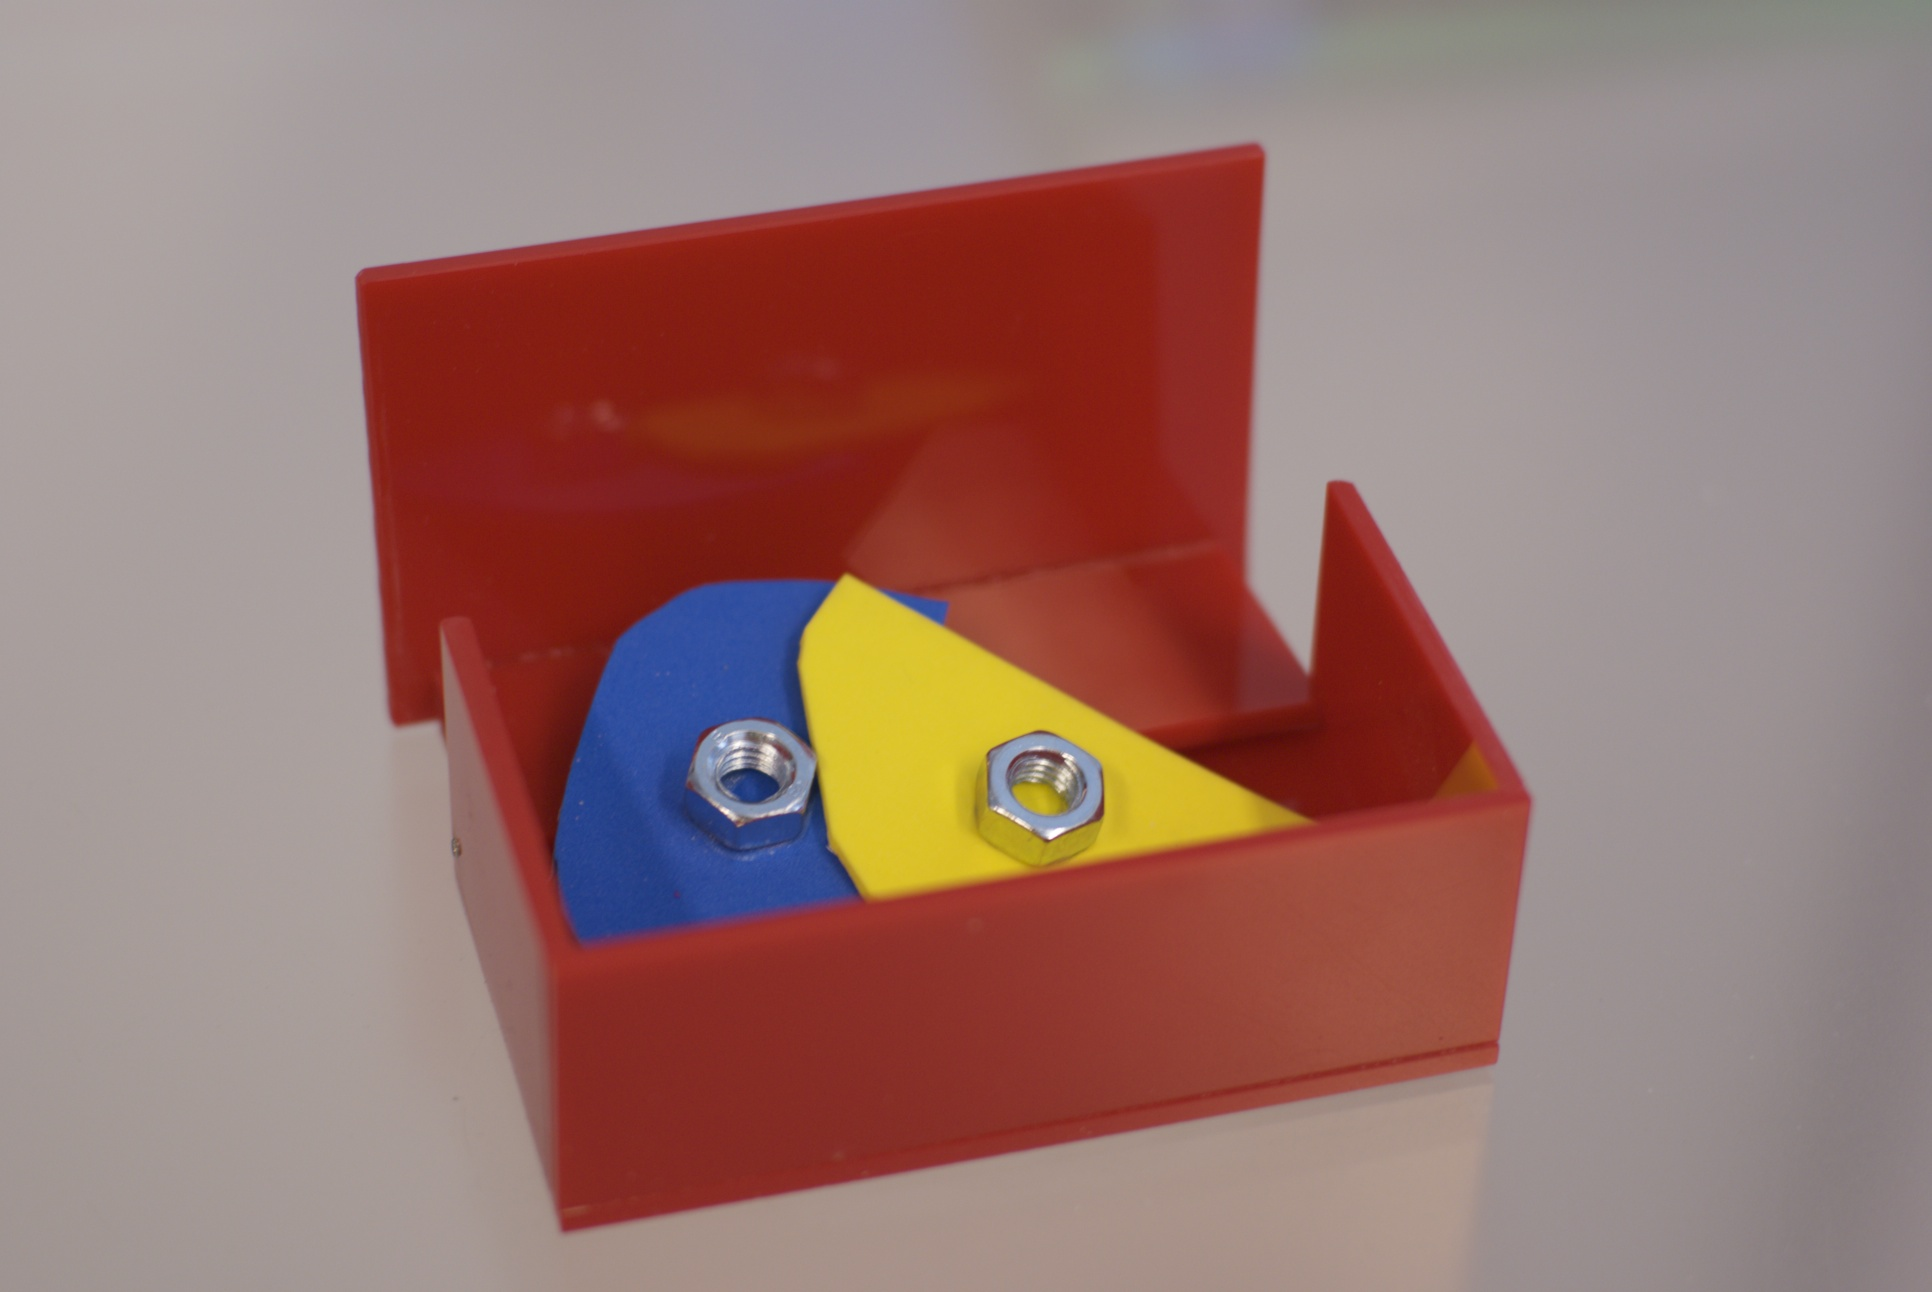
\includegraphics[height=2in]{img/ImplementierungInput/ContainerToken.jpg}
	\caption{Geöffnetes Container Token}
	\label{fig:img_ImplementierungInput_ContainerToken}
\end{figure}

% subsubsection modellierungs_tokens (end)

\subsubsection{Einbettbare Tokens} % (fold)
\label{einbettbare_tokens}



% subsubsection einbettbare_tokens (end)

\subsubsection{Werkzeug Tokens} % (fold)
\label{ssub:werkzeug_tokens}

% subsubsection werkzeug_tokens (end)
% subsection tokens_&_input_werkzeuge (end)

\subsection{Input auf der Tischoberfläche} % (fold)
\label{sub:input_auf_der_tischoberfläche}

Semitransparente Oberfläche, Projektion von unten (Umlenkspiegel), Kamera von unten - Überleitung zur 
Illumination via Interferenz zwischen Beamer und Kamera

% subsection input_auf_der_tischoberfläche (end)

\subsection{Illumination und Umgebungslichtabhängigkeit} % (fold)
\label{sub:illumination_und_umgebungslichtabhängigkeit}

% subsection illumination_und_umgebungslichtabhängigkeit (end)
% section konzeption_und_umsetzung_der_hardwarekomponenten (end)

\section{Erfassung der Benutzerinteraktion durch Software} % (fold)
\label{sec:erfassung_der_benutzerinteraktion_durch_softfware}

% section erfassung_der_benutzerinteraktion_durch_software (end)

\section{Interpretation der Rohdaten und Stabilisierung der Erkennungsleistung} % (fold)
\label{sec:interpretation_der_rohdaten_und_stabilisierung_der_erkennungsleistung}

% section interpretation_der_rohdaten_und_stabilisierung_der_erkennungsleistung (end)
% chapter input_&_interpretation (end)
